\documentclass[twoside]{book}

% Packages required by doxygen
\usepackage{calc}
\usepackage{doxygen}
\usepackage{graphicx}
\usepackage[utf8]{inputenc}
\usepackage{makeidx}
\usepackage{multicol}
\usepackage{multirow}
\usepackage{fixltx2e}
\PassOptionsToPackage{warn}{textcomp}
\usepackage{textcomp}
\usepackage[nointegrals]{wasysym}
\usepackage[table]{xcolor}

% NLS support packages
\usepackage{polski}
\usepackage[T1]{fontenc}

% Font selection
\usepackage[T1]{fontenc}
\usepackage{mathptmx}
\usepackage[scaled=.90]{helvet}
\usepackage{courier}
\usepackage{amssymb}
\usepackage{sectsty}
\renewcommand{\familydefault}{\sfdefault}
\allsectionsfont{%
  \fontseries{bc}\selectfont%
  \color{darkgray}%
}
\renewcommand{\DoxyLabelFont}{%
  \fontseries{bc}\selectfont%
  \color{darkgray}%
}
\newcommand{\+}{\discretionary{\mbox{\scriptsize$\hookleftarrow$}}{}{}}

% Page & text layout
\usepackage{geometry}
\geometry{%
  a4paper,%
  top=2.5cm,%
  bottom=2.5cm,%
  left=2.5cm,%
  right=2.5cm%
}
\tolerance=750
\hfuzz=15pt
\hbadness=750
\setlength{\emergencystretch}{15pt}
\setlength{\parindent}{0cm}
\setlength{\parskip}{0.2cm}
\makeatletter
\renewcommand{\paragraph}{%
  \@startsection{paragraph}{4}{0ex}{-1.0ex}{1.0ex}{%
    \normalfont\normalsize\bfseries\SS@parafont%
  }%
}
\renewcommand{\subparagraph}{%
  \@startsection{subparagraph}{5}{0ex}{-1.0ex}{1.0ex}{%
    \normalfont\normalsize\bfseries\SS@subparafont%
  }%
}
\makeatother

% Headers & footers
\usepackage{fancyhdr}
\pagestyle{fancyplain}
\fancyhead[LE]{\fancyplain{}{\bfseries\thepage}}
\fancyhead[CE]{\fancyplain{}{}}
\fancyhead[RE]{\fancyplain{}{\bfseries\leftmark}}
\fancyhead[LO]{\fancyplain{}{\bfseries\rightmark}}
\fancyhead[CO]{\fancyplain{}{}}
\fancyhead[RO]{\fancyplain{}{\bfseries\thepage}}
\fancyfoot[LE]{\fancyplain{}{}}
\fancyfoot[CE]{\fancyplain{}{}}
\fancyfoot[RE]{\fancyplain{}{\bfseries\scriptsize Wygenerowano Śr, 14 maj 2014 17\+:03\+:07 dla My Project programem Doxygen }}
\fancyfoot[LO]{\fancyplain{}{\bfseries\scriptsize Wygenerowano Śr, 14 maj 2014 17\+:03\+:07 dla My Project programem Doxygen }}
\fancyfoot[CO]{\fancyplain{}{}}
\fancyfoot[RO]{\fancyplain{}{}}
\renewcommand{\footrulewidth}{0.4pt}
\renewcommand{\chaptermark}[1]{%
  \markboth{#1}{}%
}
\renewcommand{\sectionmark}[1]{%
  \markright{\thesection\ #1}%
}

% Indices & bibliography
\usepackage{natbib}
\usepackage[titles]{tocloft}
\setcounter{tocdepth}{3}
\setcounter{secnumdepth}{5}
\makeindex

% Hyperlinks (required, but should be loaded last)
\usepackage{ifpdf}
\ifpdf
  \usepackage[pdftex,pagebackref=true]{hyperref}
\else
  \usepackage[ps2pdf,pagebackref=true]{hyperref}
\fi
\hypersetup{%
  colorlinks=true,%
  linkcolor=blue,%
  citecolor=blue,%
  unicode%
}

% Custom commands
\newcommand{\clearemptydoublepage}{%
  \newpage{\pagestyle{empty}\cleardoublepage}%
}


%===== C O N T E N T S =====

\begin{document}

% Titlepage & ToC
\hypersetup{pageanchor=false,
             bookmarks=true,
             bookmarksnumbered=true,
             pdfencoding=unicode
            }
\pagenumbering{roman}
\begin{titlepage}
\vspace*{7cm}
\begin{center}%
{\Large My Project }\\
\vspace*{1cm}
{\large Wygenerowano przez Doxygen 1.8.7}\\
\vspace*{0.5cm}
{\small Śr, 14 maj 2014 17:03:07}\\
\end{center}
\end{titlepage}
\clearemptydoublepage
\tableofcontents
\clearemptydoublepage
\pagenumbering{arabic}
\hypersetup{pageanchor=true}

%--- Begin generated contents ---
\chapter{Indeks przestrzeni nazw}
\section{Pakiety}
Oto lista pakietów wraz z krótkim opisem (o ile jest dostępny)\+:\begin{DoxyCompactList}
\item\contentsline{section}{\hyperlink{namespace_smart__install}{Smart\+\_\+install} }{\pageref{namespace_smart__install}}{}
\end{DoxyCompactList}

\chapter{Indeks hierarchiczny}
\section{Hierarchia klas}
Ta lista dziedziczenia posortowana jest z grubsza, choć nie całkowicie, alfabetycznie\+:\begin{DoxyCompactList}
\item \contentsline{section}{Smart\+\_\+install.\+Archive}{\pageref{class_smart__install_1_1_archive}}{}
\item \contentsline{section}{Smart\+\_\+install.\+archive\+Information}{\pageref{class_smart__install_1_1archive_information}}{}
\item \contentsline{section}{Smart\+\_\+install.\+control}{\pageref{class_smart__install_1_1control}}{}
\item Db\+Context\begin{DoxyCompactList}
\item \contentsline{section}{Smart\+\_\+install.\+Archive\+Base\+Entities2}{\pageref{class_smart__install_1_1_archive_base_entities2}}{}
\end{DoxyCompactList}
\item \contentsline{section}{Smart\+\_\+install.\+Exec}{\pageref{class_smart__install_1_1_exec}}{}
\item Form\begin{DoxyCompactList}
\item \contentsline{section}{Smart\+\_\+install.\+Add\+Programs}{\pageref{class_smart__install_1_1_add_programs}}{}
\item \contentsline{section}{Smart\+\_\+install.\+Help2}{\pageref{class_smart__install_1_1_help2}}{}
\item \contentsline{section}{Smart\+\_\+install.\+Menu\+Install}{\pageref{class_smart__install_1_1_menu_install}}{}
\item \contentsline{section}{Smart\+\_\+install.\+New\+Arch}{\pageref{class_smart__install_1_1_new_arch}}{}
\item \contentsline{section}{Smart\+\_\+install.\+user\+Menu\+Install}{\pageref{class_smart__install_1_1user_menu_install}}{}
\end{DoxyCompactList}
\item \contentsline{section}{Smart\+\_\+install.\+Search\+Program.\+Install\+Program}{\pageref{struct_smart__install_1_1_search_program_1_1_install_program}}{}
\item \contentsline{section}{Smart\+\_\+install.\+Language}{\pageref{class_smart__install_1_1_language}}{}
\item \contentsline{section}{Smart\+\_\+install.\+Prog}{\pageref{class_smart__install_1_1_prog}}{}
\item \contentsline{section}{Smart\+\_\+install.\+program\+Information}{\pageref{class_smart__install_1_1program_information}}{}
\item \contentsline{section}{Smart\+\_\+install.\+Search\+Program}{\pageref{class_smart__install_1_1_search_program}}{}
\item \contentsline{section}{Smart\+\_\+install.\+system\+Type}{\pageref{class_smart__install_1_1system_type}}{}
\item \contentsline{section}{Smart\+\_\+install.\+Tag}{\pageref{class_smart__install_1_1_tag}}{}
\item \contentsline{section}{Smart\+\_\+install.\+zip\+Creator}{\pageref{class_smart__install_1_1zip_creator}}{}
\end{DoxyCompactList}

\chapter{Indeks klas}
\section{Lista klas}
Tutaj znajdują się klasy, struktury, unie i interfejsy wraz z ich krótkimi opisami\+:\begin{DoxyCompactList}
\item\contentsline{section}{\hyperlink{class_smart__install_1_1_add_programs}{Smart\+\_\+install.\+Add\+Programs} }{\pageref{class_smart__install_1_1_add_programs}}{}
\item\contentsline{section}{\hyperlink{class_smart__install_1_1_archive}{Smart\+\_\+install.\+Archive} }{\pageref{class_smart__install_1_1_archive}}{}
\item\contentsline{section}{\hyperlink{class_smart__install_1_1_archive_base_entities2}{Smart\+\_\+install.\+Archive\+Base\+Entities2} }{\pageref{class_smart__install_1_1_archive_base_entities2}}{}
\item\contentsline{section}{\hyperlink{class_smart__install_1_1archive_information}{Smart\+\_\+install.\+archive\+Information} \\*Klasa reprezentująca informację na temat archiwum uzyskiwane od urzytkownika }{\pageref{class_smart__install_1_1archive_information}}{}
\item\contentsline{section}{\hyperlink{class_smart__install_1_1control}{Smart\+\_\+install.\+control} }{\pageref{class_smart__install_1_1control}}{}
\item\contentsline{section}{\hyperlink{class_smart__install_1_1_exec}{Smart\+\_\+install.\+Exec} }{\pageref{class_smart__install_1_1_exec}}{}
\item\contentsline{section}{\hyperlink{class_smart__install_1_1_help2}{Smart\+\_\+install.\+Help2} }{\pageref{class_smart__install_1_1_help2}}{}
\item\contentsline{section}{\hyperlink{struct_smart__install_1_1_search_program_1_1_install_program}{Smart\+\_\+install.\+Search\+Program.\+Install\+Program} }{\pageref{struct_smart__install_1_1_search_program_1_1_install_program}}{}
\item\contentsline{section}{\hyperlink{class_smart__install_1_1_language}{Smart\+\_\+install.\+Language} }{\pageref{class_smart__install_1_1_language}}{}
\item\contentsline{section}{\hyperlink{class_smart__install_1_1_menu_install}{Smart\+\_\+install.\+Menu\+Install} }{\pageref{class_smart__install_1_1_menu_install}}{}
\item\contentsline{section}{\hyperlink{class_smart__install_1_1_new_arch}{Smart\+\_\+install.\+New\+Arch} }{\pageref{class_smart__install_1_1_new_arch}}{}
\item\contentsline{section}{\hyperlink{class_smart__install_1_1_prog}{Smart\+\_\+install.\+Prog} }{\pageref{class_smart__install_1_1_prog}}{}
\item\contentsline{section}{\hyperlink{class_smart__install_1_1program_information}{Smart\+\_\+install.\+program\+Information} \\*Klasa reprezentująca informację na temat programu uzyskiwane od użytkownika }{\pageref{class_smart__install_1_1program_information}}{}
\item\contentsline{section}{\hyperlink{class_smart__install_1_1_search_program}{Smart\+\_\+install.\+Search\+Program} }{\pageref{class_smart__install_1_1_search_program}}{}
\item\contentsline{section}{\hyperlink{class_smart__install_1_1system_type}{Smart\+\_\+install.\+system\+Type} }{\pageref{class_smart__install_1_1system_type}}{}
\item\contentsline{section}{\hyperlink{class_smart__install_1_1_tag}{Smart\+\_\+install.\+Tag} }{\pageref{class_smart__install_1_1_tag}}{}
\item\contentsline{section}{\hyperlink{class_smart__install_1_1user_menu_install}{Smart\+\_\+install.\+user\+Menu\+Install} }{\pageref{class_smart__install_1_1user_menu_install}}{}
\item\contentsline{section}{\hyperlink{class_smart__install_1_1zip_creator}{Smart\+\_\+install.\+zip\+Creator} }{\pageref{class_smart__install_1_1zip_creator}}{}
\end{DoxyCompactList}

\chapter{Indeks plików}
\section{Lista plików}
Tutaj znajduje się lista wszystkich plików z ich krótkimi opisami\+:\begin{DoxyCompactList}
\item\contentsline{section}{\hyperlink{_add_programs_8cs}{Add\+Programs.\+cs} }{\pageref{_add_programs_8cs}}{}
\item\contentsline{section}{\hyperlink{_add_programs_8_designer_8cs}{Add\+Programs.\+Designer.\+cs} }{\pageref{_add_programs_8_designer_8cs}}{}
\item\contentsline{section}{\hyperlink{_archive_8cs}{Archive.\+cs} }{\pageref{_archive_8cs}}{}
\item\contentsline{section}{\hyperlink{control_8cs}{control.\+cs} }{\pageref{control_8cs}}{}
\item\contentsline{section}{\hyperlink{_exec_8cs}{Exec.\+cs} }{\pageref{_exec_8cs}}{}
\item\contentsline{section}{\hyperlink{_help2_8cs}{Help2.\+cs} }{\pageref{_help2_8cs}}{}
\item\contentsline{section}{\hyperlink{_help2_8_designer_8cs}{Help2.\+Designer.\+cs} }{\pageref{_help2_8_designer_8cs}}{}
\item\contentsline{section}{\hyperlink{_language_8cs}{Language.\+cs} }{\pageref{_language_8cs}}{}
\item\contentsline{section}{\hyperlink{_menu_install_8cs}{Menu\+Install.\+cs} }{\pageref{_menu_install_8cs}}{}
\item\contentsline{section}{\hyperlink{_menu_install_8_designer_8cs}{Menu\+Install.\+Designer.\+cs} }{\pageref{_menu_install_8_designer_8cs}}{}
\item\contentsline{section}{\hyperlink{_model_archive_8_context_8cs}{Model\+Archive.\+Context.\+cs} }{\pageref{_model_archive_8_context_8cs}}{}
\item\contentsline{section}{\hyperlink{_model_archive_8cs}{Model\+Archive.\+cs} }{\pageref{_model_archive_8cs}}{}
\item\contentsline{section}{\hyperlink{_model_archive_8_designer_8cs}{Model\+Archive.\+Designer.\+cs} }{\pageref{_model_archive_8_designer_8cs}}{}
\item\contentsline{section}{\hyperlink{_new_arch_8cs}{New\+Arch.\+cs} }{\pageref{_new_arch_8cs}}{}
\item\contentsline{section}{\hyperlink{_new_arch_8_designer_8cs}{New\+Arch.\+Designer.\+cs} }{\pageref{_new_arch_8_designer_8cs}}{}
\item\contentsline{section}{\hyperlink{_prog_8cs}{Prog.\+cs} }{\pageref{_prog_8cs}}{}
\item\contentsline{section}{\hyperlink{_search_program_8cs}{Search\+Program.\+cs} }{\pageref{_search_program_8cs}}{}
\item\contentsline{section}{\hyperlink{system_type_8cs}{system\+Type.\+cs} }{\pageref{system_type_8cs}}{}
\item\contentsline{section}{\hyperlink{_tag_8cs}{Tag.\+cs} }{\pageref{_tag_8cs}}{}
\item\contentsline{section}{\hyperlink{user_menu_install_8cs}{user\+Menu\+Install.\+cs} }{\pageref{user_menu_install_8cs}}{}
\item\contentsline{section}{\hyperlink{user_menu_install_8_designer_8cs}{user\+Menu\+Install.\+Designer.\+cs} }{\pageref{user_menu_install_8_designer_8cs}}{}
\item\contentsline{section}{\hyperlink{zip_creator_8cs}{zip\+Creator.\+cs} }{\pageref{zip_creator_8cs}}{}
\end{DoxyCompactList}

\chapter{Dokumentacja przestrzeni nazw}
\hypertarget{namespace_smart__install}{\section{Pakiet Smart\+\_\+install}
\label{namespace_smart__install}\index{Smart\+\_\+install@{Smart\+\_\+install}}
}
\subsection*{Komponenty}
\begin{DoxyCompactItemize}
\item 
class \hyperlink{class_smart__install_1_1_add_programs}{Add\+Programs}
\item 
class \hyperlink{class_smart__install_1_1_archive}{Archive}
\item 
class \hyperlink{class_smart__install_1_1_archive_base_entities2}{Archive\+Base\+Entities2}
\item 
class \hyperlink{class_smart__install_1_1archive_information}{archive\+Information}
\begin{DoxyCompactList}\small\item\em Klasa reprezentująca informację na temat archiwum uzyskiwane od urzytkownika \end{DoxyCompactList}\item 
class \hyperlink{class_smart__install_1_1control}{control}
\item 
class \hyperlink{class_smart__install_1_1_exec}{Exec}
\item 
class \hyperlink{class_smart__install_1_1_help2}{Help2}
\item 
class \hyperlink{class_smart__install_1_1_language}{Language}
\item 
class \hyperlink{class_smart__install_1_1_menu_install}{Menu\+Install}
\item 
class \hyperlink{class_smart__install_1_1_new_arch}{New\+Arch}
\item 
class \hyperlink{class_smart__install_1_1_prog}{Prog}
\item 
class \hyperlink{class_smart__install_1_1program_information}{program\+Information}
\begin{DoxyCompactList}\small\item\em Klasa reprezentująca informację na temat programu uzyskiwane od użytkownika \end{DoxyCompactList}\item 
class \hyperlink{class_smart__install_1_1_search_program}{Search\+Program}
\item 
class \hyperlink{class_smart__install_1_1system_type}{system\+Type}
\item 
class \hyperlink{class_smart__install_1_1_tag}{Tag}
\item 
class \hyperlink{class_smart__install_1_1user_menu_install}{user\+Menu\+Install}
\item 
class \hyperlink{class_smart__install_1_1zip_creator}{zip\+Creator}
\end{DoxyCompactItemize}

\chapter{Dokumentacja klas}
\hypertarget{class_smart__install_1_1_add_programs}{\section{Dokumentacja klasy Smart\+\_\+install.\+Add\+Programs}
\label{class_smart__install_1_1_add_programs}\index{Smart\+\_\+install.\+Add\+Programs@{Smart\+\_\+install.\+Add\+Programs}}
}
Diagram dziedziczenia dla Smart\+\_\+install.\+Add\+Programs\begin{figure}[H]
\begin{center}
\leavevmode
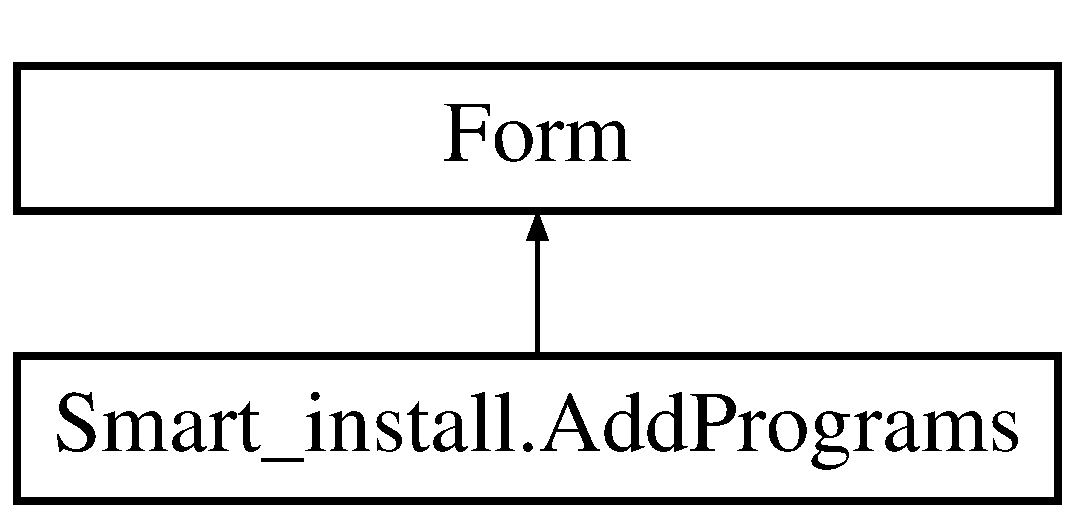
\includegraphics[height=2.000000cm]{class_smart__install_1_1_add_programs}
\end{center}
\end{figure}
\subsection*{Metody publiczne}
\begin{DoxyCompactItemize}
\item 
\hyperlink{class_smart__install_1_1_add_programs_a5dca12781a08d230249af4519626435d}{Add\+Programs} (string Path, \hyperlink{class_smart__install_1_1_new_arch}{New\+Arch} parent)
\item 
\hyperlink{class_smart__install_1_1_add_programs_aeb43ce91c812f52325913bc3ef697a31}{Add\+Programs} (\hyperlink{class_smart__install_1_1program_information}{program\+Information} first\+Program, \hyperlink{class_smart__install_1_1_new_arch}{New\+Arch} parent)
\end{DoxyCompactItemize}
\subsection*{Metody chronione}
\begin{DoxyCompactItemize}
\item 
override void \hyperlink{class_smart__install_1_1_add_programs_afd32b6bfead4212758a97864bf47e0d0}{Dispose} (bool disposing)
\begin{DoxyCompactList}\small\item\em Clean up any resources being used. \end{DoxyCompactList}\end{DoxyCompactItemize}


\subsection{Opis szczegółowy}


Definicja w linii 13 pliku Add\+Programs.\+cs.



\subsection{Dokumentacja konstruktora i destruktora}
\hypertarget{class_smart__install_1_1_add_programs_a5dca12781a08d230249af4519626435d}{\index{Smart\+\_\+install\+::\+Add\+Programs@{Smart\+\_\+install\+::\+Add\+Programs}!Add\+Programs@{Add\+Programs}}
\index{Add\+Programs@{Add\+Programs}!Smart\+\_\+install\+::\+Add\+Programs@{Smart\+\_\+install\+::\+Add\+Programs}}
\subsubsection[{Add\+Programs}]{\setlength{\rightskip}{0pt plus 5cm}Smart\+\_\+install.\+Add\+Programs.\+Add\+Programs (
\begin{DoxyParamCaption}
\item[{string}]{Path, }
\item[{{\bf New\+Arch}}]{parent}
\end{DoxyParamCaption}
)}}\label{class_smart__install_1_1_add_programs_a5dca12781a08d230249af4519626435d}


Definicja w linii 22 pliku Add\+Programs.\+cs.

\hypertarget{class_smart__install_1_1_add_programs_aeb43ce91c812f52325913bc3ef697a31}{\index{Smart\+\_\+install\+::\+Add\+Programs@{Smart\+\_\+install\+::\+Add\+Programs}!Add\+Programs@{Add\+Programs}}
\index{Add\+Programs@{Add\+Programs}!Smart\+\_\+install\+::\+Add\+Programs@{Smart\+\_\+install\+::\+Add\+Programs}}
\subsubsection[{Add\+Programs}]{\setlength{\rightskip}{0pt plus 5cm}Smart\+\_\+install.\+Add\+Programs.\+Add\+Programs (
\begin{DoxyParamCaption}
\item[{{\bf program\+Information}}]{first\+Program, }
\item[{{\bf New\+Arch}}]{parent}
\end{DoxyParamCaption}
)}}\label{class_smart__install_1_1_add_programs_aeb43ce91c812f52325913bc3ef697a31}


Definicja w linii 46 pliku Add\+Programs.\+cs.



\subsection{Dokumentacja funkcji składowych}
\hypertarget{class_smart__install_1_1_add_programs_afd32b6bfead4212758a97864bf47e0d0}{\index{Smart\+\_\+install\+::\+Add\+Programs@{Smart\+\_\+install\+::\+Add\+Programs}!Dispose@{Dispose}}
\index{Dispose@{Dispose}!Smart\+\_\+install\+::\+Add\+Programs@{Smart\+\_\+install\+::\+Add\+Programs}}
\subsubsection[{Dispose}]{\setlength{\rightskip}{0pt plus 5cm}override void Smart\+\_\+install.\+Add\+Programs.\+Dispose (
\begin{DoxyParamCaption}
\item[{bool}]{disposing}
\end{DoxyParamCaption}
)\hspace{0.3cm}{\ttfamily [protected]}}}\label{class_smart__install_1_1_add_programs_afd32b6bfead4212758a97864bf47e0d0}


Clean up any resources being used. 


\begin{DoxyParams}{Parametry}
{\em disposing} & true if managed resources should be disposed; otherwise, false.\\
\hline
\end{DoxyParams}


Definicja w linii 14 pliku Add\+Programs.\+Designer.\+cs.



Dokumentacja dla tej klasy została wygenerowana z plików\+:\begin{DoxyCompactItemize}
\item 
\hyperlink{_add_programs_8cs}{Add\+Programs.\+cs}\item 
\hyperlink{_add_programs_8_designer_8cs}{Add\+Programs.\+Designer.\+cs}\end{DoxyCompactItemize}

\hypertarget{class_smart__install_1_1_archive}{\section{Dokumentacja klasy Smart\+\_\+install.\+Archive}
\label{class_smart__install_1_1_archive}\index{Smart\+\_\+install.\+Archive@{Smart\+\_\+install.\+Archive}}
}
\subsection*{Metody publiczne}
\begin{DoxyCompactItemize}
\item 
\hyperlink{class_smart__install_1_1_archive_a82cb112c00eda77255937ffb038c90d8}{Archive} ()
\end{DoxyCompactItemize}
\subsection*{Właściwości}
\begin{DoxyCompactItemize}
\item 
int \hyperlink{class_smart__install_1_1_archive_afd080039becc9c704f1d4d2cd8e590f3}{Id}\hspace{0.3cm}{\ttfamily  \mbox{[}get, set\mbox{]}}
\item 
string \hyperlink{class_smart__install_1_1_archive_ab2a5b01802980603eac526169f0f4366}{Name}\hspace{0.3cm}{\ttfamily  \mbox{[}get, set\mbox{]}}
\item 
string \hyperlink{class_smart__install_1_1_archive_a40e8f14a943da30b52300495888eab9a}{Path}\hspace{0.3cm}{\ttfamily  \mbox{[}get, set\mbox{]}}
\item 
Nullable$<$ System.\+Date\+Time $>$ \hyperlink{class_smart__install_1_1_archive_a6eb9ecd6f2c8a25d62e509ed46e69621}{Create\+Date}\hspace{0.3cm}{\ttfamily  \mbox{[}get, set\mbox{]}}
\item 
Nullable$<$ System.\+Date\+Time $>$ \hyperlink{class_smart__install_1_1_archive_abd1dc9feb078ec7db9e3f63fef8a3db6}{Modified\+Date}\hspace{0.3cm}{\ttfamily  \mbox{[}get, set\mbox{]}}
\item 
string \hyperlink{class_smart__install_1_1_archive_ae39bf3c2778783c5c68ad0e8a5b0e966}{Description}\hspace{0.3cm}{\ttfamily  \mbox{[}get, set\mbox{]}}
\item 
virtual I\+Collection$<$ \hyperlink{class_smart__install_1_1_prog}{Prog} $>$ \hyperlink{class_smart__install_1_1_archive_aee224a0c3036cd495e63818a2efa4218}{Progs}\hspace{0.3cm}{\ttfamily  \mbox{[}get, set\mbox{]}}
\end{DoxyCompactItemize}


\subsection{Opis szczegółowy}


Definicja w linii 15 pliku Archive.\+cs.



\subsection{Dokumentacja konstruktora i destruktora}
\hypertarget{class_smart__install_1_1_archive_a82cb112c00eda77255937ffb038c90d8}{\index{Smart\+\_\+install\+::\+Archive@{Smart\+\_\+install\+::\+Archive}!Archive@{Archive}}
\index{Archive@{Archive}!Smart\+\_\+install\+::\+Archive@{Smart\+\_\+install\+::\+Archive}}
\subsubsection[{Archive}]{\setlength{\rightskip}{0pt plus 5cm}Smart\+\_\+install.\+Archive.\+Archive (
\begin{DoxyParamCaption}
{}
\end{DoxyParamCaption}
)}}\label{class_smart__install_1_1_archive_a82cb112c00eda77255937ffb038c90d8}


Definicja w linii 17 pliku Archive.\+cs.



\subsection{Dokumentacja właściwości}
\hypertarget{class_smart__install_1_1_archive_a6eb9ecd6f2c8a25d62e509ed46e69621}{\index{Smart\+\_\+install\+::\+Archive@{Smart\+\_\+install\+::\+Archive}!Create\+Date@{Create\+Date}}
\index{Create\+Date@{Create\+Date}!Smart\+\_\+install\+::\+Archive@{Smart\+\_\+install\+::\+Archive}}
\subsubsection[{Create\+Date}]{\setlength{\rightskip}{0pt plus 5cm}Nullable$<$System.\+Date\+Time$>$ Smart\+\_\+install.\+Archive.\+Create\+Date\hspace{0.3cm}{\ttfamily [get]}, {\ttfamily [set]}}}\label{class_smart__install_1_1_archive_a6eb9ecd6f2c8a25d62e509ed46e69621}


Definicja w linii 25 pliku Archive.\+cs.

\hypertarget{class_smart__install_1_1_archive_ae39bf3c2778783c5c68ad0e8a5b0e966}{\index{Smart\+\_\+install\+::\+Archive@{Smart\+\_\+install\+::\+Archive}!Description@{Description}}
\index{Description@{Description}!Smart\+\_\+install\+::\+Archive@{Smart\+\_\+install\+::\+Archive}}
\subsubsection[{Description}]{\setlength{\rightskip}{0pt plus 5cm}string Smart\+\_\+install.\+Archive.\+Description\hspace{0.3cm}{\ttfamily [get]}, {\ttfamily [set]}}}\label{class_smart__install_1_1_archive_ae39bf3c2778783c5c68ad0e8a5b0e966}


Definicja w linii 27 pliku Archive.\+cs.

\hypertarget{class_smart__install_1_1_archive_afd080039becc9c704f1d4d2cd8e590f3}{\index{Smart\+\_\+install\+::\+Archive@{Smart\+\_\+install\+::\+Archive}!Id@{Id}}
\index{Id@{Id}!Smart\+\_\+install\+::\+Archive@{Smart\+\_\+install\+::\+Archive}}
\subsubsection[{Id}]{\setlength{\rightskip}{0pt plus 5cm}int Smart\+\_\+install.\+Archive.\+Id\hspace{0.3cm}{\ttfamily [get]}, {\ttfamily [set]}}}\label{class_smart__install_1_1_archive_afd080039becc9c704f1d4d2cd8e590f3}


Definicja w linii 22 pliku Archive.\+cs.

\hypertarget{class_smart__install_1_1_archive_abd1dc9feb078ec7db9e3f63fef8a3db6}{\index{Smart\+\_\+install\+::\+Archive@{Smart\+\_\+install\+::\+Archive}!Modified\+Date@{Modified\+Date}}
\index{Modified\+Date@{Modified\+Date}!Smart\+\_\+install\+::\+Archive@{Smart\+\_\+install\+::\+Archive}}
\subsubsection[{Modified\+Date}]{\setlength{\rightskip}{0pt plus 5cm}Nullable$<$System.\+Date\+Time$>$ Smart\+\_\+install.\+Archive.\+Modified\+Date\hspace{0.3cm}{\ttfamily [get]}, {\ttfamily [set]}}}\label{class_smart__install_1_1_archive_abd1dc9feb078ec7db9e3f63fef8a3db6}


Definicja w linii 26 pliku Archive.\+cs.

\hypertarget{class_smart__install_1_1_archive_ab2a5b01802980603eac526169f0f4366}{\index{Smart\+\_\+install\+::\+Archive@{Smart\+\_\+install\+::\+Archive}!Name@{Name}}
\index{Name@{Name}!Smart\+\_\+install\+::\+Archive@{Smart\+\_\+install\+::\+Archive}}
\subsubsection[{Name}]{\setlength{\rightskip}{0pt plus 5cm}string Smart\+\_\+install.\+Archive.\+Name\hspace{0.3cm}{\ttfamily [get]}, {\ttfamily [set]}}}\label{class_smart__install_1_1_archive_ab2a5b01802980603eac526169f0f4366}


Definicja w linii 23 pliku Archive.\+cs.

\hypertarget{class_smart__install_1_1_archive_a40e8f14a943da30b52300495888eab9a}{\index{Smart\+\_\+install\+::\+Archive@{Smart\+\_\+install\+::\+Archive}!Path@{Path}}
\index{Path@{Path}!Smart\+\_\+install\+::\+Archive@{Smart\+\_\+install\+::\+Archive}}
\subsubsection[{Path}]{\setlength{\rightskip}{0pt plus 5cm}string Smart\+\_\+install.\+Archive.\+Path\hspace{0.3cm}{\ttfamily [get]}, {\ttfamily [set]}}}\label{class_smart__install_1_1_archive_a40e8f14a943da30b52300495888eab9a}


Definicja w linii 24 pliku Archive.\+cs.

\hypertarget{class_smart__install_1_1_archive_aee224a0c3036cd495e63818a2efa4218}{\index{Smart\+\_\+install\+::\+Archive@{Smart\+\_\+install\+::\+Archive}!Progs@{Progs}}
\index{Progs@{Progs}!Smart\+\_\+install\+::\+Archive@{Smart\+\_\+install\+::\+Archive}}
\subsubsection[{Progs}]{\setlength{\rightskip}{0pt plus 5cm}virtual I\+Collection$<${\bf Prog}$>$ Smart\+\_\+install.\+Archive.\+Progs\hspace{0.3cm}{\ttfamily [get]}, {\ttfamily [set]}}}\label{class_smart__install_1_1_archive_aee224a0c3036cd495e63818a2efa4218}


Definicja w linii 29 pliku Archive.\+cs.



Dokumentacja dla tej klasy została wygenerowana z pliku\+:\begin{DoxyCompactItemize}
\item 
\hyperlink{_archive_8cs}{Archive.\+cs}\end{DoxyCompactItemize}

\hypertarget{class_smart__install_1_1_archive_base_entities2}{\section{Dokumentacja klasy Smart\+\_\+install.\+Archive\+Base\+Entities2}
\label{class_smart__install_1_1_archive_base_entities2}\index{Smart\+\_\+install.\+Archive\+Base\+Entities2@{Smart\+\_\+install.\+Archive\+Base\+Entities2}}
}
Diagram dziedziczenia dla Smart\+\_\+install.\+Archive\+Base\+Entities2\begin{figure}[H]
\begin{center}
\leavevmode
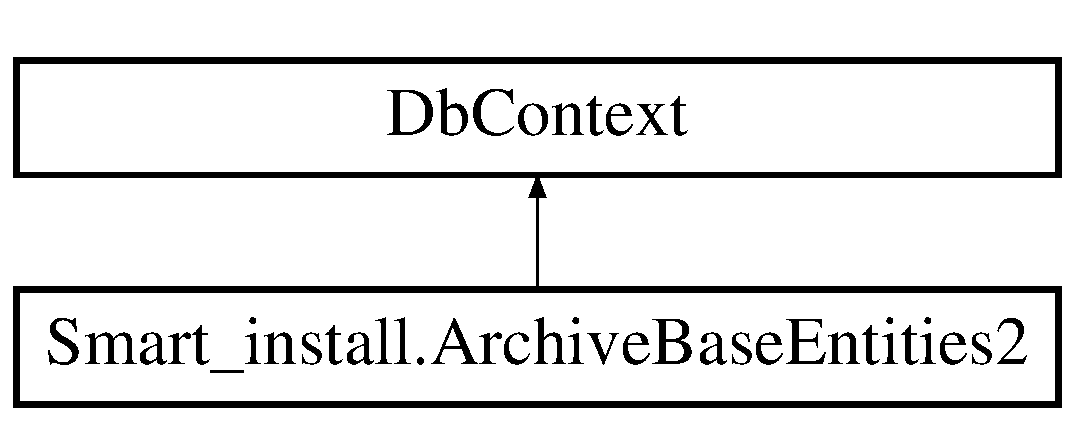
\includegraphics[height=2.000000cm]{class_smart__install_1_1_archive_base_entities2}
\end{center}
\end{figure}
\subsection*{Metody publiczne}
\begin{DoxyCompactItemize}
\item 
\hyperlink{class_smart__install_1_1_archive_base_entities2_a9ca605fc5a79dc61bdeafa0a6588664a}{Archive\+Base\+Entities2} ()
\end{DoxyCompactItemize}
\subsection*{Metody chronione}
\begin{DoxyCompactItemize}
\item 
override void \hyperlink{class_smart__install_1_1_archive_base_entities2_af346b2a15acf04656b64b4c570a15363}{On\+Model\+Creating} (Db\+Model\+Builder model\+Builder)
\end{DoxyCompactItemize}
\subsection*{Właściwości}
\begin{DoxyCompactItemize}
\item 
Db\+Set$<$ \hyperlink{class_smart__install_1_1_archive}{Archive} $>$ \hyperlink{class_smart__install_1_1_archive_base_entities2_a405bbf0b59d84859ee55e7667f9914eb}{Archives}\hspace{0.3cm}{\ttfamily  \mbox{[}get, set\mbox{]}}
\item 
Db\+Set$<$ \hyperlink{class_smart__install_1_1_language}{Language} $>$ \hyperlink{class_smart__install_1_1_archive_base_entities2_aa44a1546a9fbf51f1c599f772e8a1aa3}{Languages}\hspace{0.3cm}{\ttfamily  \mbox{[}get, set\mbox{]}}
\item 
Db\+Set$<$ \hyperlink{class_smart__install_1_1_prog}{Prog} $>$ \hyperlink{class_smart__install_1_1_archive_base_entities2_a70a23976dcecf46e3f71b19e6a02a723}{Progs}\hspace{0.3cm}{\ttfamily  \mbox{[}get, set\mbox{]}}
\item 
Db\+Set$<$ \hyperlink{class_smart__install_1_1system_type}{system\+Type} $>$ \hyperlink{class_smart__install_1_1_archive_base_entities2_a2d740959abb28124acc90d6a8eb4fdd9}{system\+Types}\hspace{0.3cm}{\ttfamily  \mbox{[}get, set\mbox{]}}
\item 
Db\+Set$<$ \hyperlink{class_smart__install_1_1_tag}{Tag} $>$ \hyperlink{class_smart__install_1_1_archive_base_entities2_aec8c3eec718e967babe00f42e4988996}{Tags}\hspace{0.3cm}{\ttfamily  \mbox{[}get, set\mbox{]}}
\end{DoxyCompactItemize}


\subsection{Opis szczegółowy}


Definicja w linii 16 pliku Model\+Archive.\+Context.\+cs.



\subsection{Dokumentacja konstruktora i destruktora}
\hypertarget{class_smart__install_1_1_archive_base_entities2_a9ca605fc5a79dc61bdeafa0a6588664a}{\index{Smart\+\_\+install\+::\+Archive\+Base\+Entities2@{Smart\+\_\+install\+::\+Archive\+Base\+Entities2}!Archive\+Base\+Entities2@{Archive\+Base\+Entities2}}
\index{Archive\+Base\+Entities2@{Archive\+Base\+Entities2}!Smart\+\_\+install\+::\+Archive\+Base\+Entities2@{Smart\+\_\+install\+::\+Archive\+Base\+Entities2}}
\subsubsection[{Archive\+Base\+Entities2}]{\setlength{\rightskip}{0pt plus 5cm}Smart\+\_\+install.\+Archive\+Base\+Entities2.\+Archive\+Base\+Entities2 (
\begin{DoxyParamCaption}
{}
\end{DoxyParamCaption}
)}}\label{class_smart__install_1_1_archive_base_entities2_a9ca605fc5a79dc61bdeafa0a6588664a}


Definicja w linii 18 pliku Model\+Archive.\+Context.\+cs.



\subsection{Dokumentacja funkcji składowych}
\hypertarget{class_smart__install_1_1_archive_base_entities2_af346b2a15acf04656b64b4c570a15363}{\index{Smart\+\_\+install\+::\+Archive\+Base\+Entities2@{Smart\+\_\+install\+::\+Archive\+Base\+Entities2}!On\+Model\+Creating@{On\+Model\+Creating}}
\index{On\+Model\+Creating@{On\+Model\+Creating}!Smart\+\_\+install\+::\+Archive\+Base\+Entities2@{Smart\+\_\+install\+::\+Archive\+Base\+Entities2}}
\subsubsection[{On\+Model\+Creating}]{\setlength{\rightskip}{0pt plus 5cm}override void Smart\+\_\+install.\+Archive\+Base\+Entities2.\+On\+Model\+Creating (
\begin{DoxyParamCaption}
\item[{Db\+Model\+Builder}]{model\+Builder}
\end{DoxyParamCaption}
)\hspace{0.3cm}{\ttfamily [protected]}}}\label{class_smart__install_1_1_archive_base_entities2_af346b2a15acf04656b64b4c570a15363}


Definicja w linii 23 pliku Model\+Archive.\+Context.\+cs.



\subsection{Dokumentacja właściwości}
\hypertarget{class_smart__install_1_1_archive_base_entities2_a405bbf0b59d84859ee55e7667f9914eb}{\index{Smart\+\_\+install\+::\+Archive\+Base\+Entities2@{Smart\+\_\+install\+::\+Archive\+Base\+Entities2}!Archives@{Archives}}
\index{Archives@{Archives}!Smart\+\_\+install\+::\+Archive\+Base\+Entities2@{Smart\+\_\+install\+::\+Archive\+Base\+Entities2}}
\subsubsection[{Archives}]{\setlength{\rightskip}{0pt plus 5cm}Db\+Set$<${\bf Archive}$>$ Smart\+\_\+install.\+Archive\+Base\+Entities2.\+Archives\hspace{0.3cm}{\ttfamily [get]}, {\ttfamily [set]}}}\label{class_smart__install_1_1_archive_base_entities2_a405bbf0b59d84859ee55e7667f9914eb}


Definicja w linii 28 pliku Model\+Archive.\+Context.\+cs.

\hypertarget{class_smart__install_1_1_archive_base_entities2_aa44a1546a9fbf51f1c599f772e8a1aa3}{\index{Smart\+\_\+install\+::\+Archive\+Base\+Entities2@{Smart\+\_\+install\+::\+Archive\+Base\+Entities2}!Languages@{Languages}}
\index{Languages@{Languages}!Smart\+\_\+install\+::\+Archive\+Base\+Entities2@{Smart\+\_\+install\+::\+Archive\+Base\+Entities2}}
\subsubsection[{Languages}]{\setlength{\rightskip}{0pt plus 5cm}Db\+Set$<${\bf Language}$>$ Smart\+\_\+install.\+Archive\+Base\+Entities2.\+Languages\hspace{0.3cm}{\ttfamily [get]}, {\ttfamily [set]}}}\label{class_smart__install_1_1_archive_base_entities2_aa44a1546a9fbf51f1c599f772e8a1aa3}


Definicja w linii 29 pliku Model\+Archive.\+Context.\+cs.

\hypertarget{class_smart__install_1_1_archive_base_entities2_a70a23976dcecf46e3f71b19e6a02a723}{\index{Smart\+\_\+install\+::\+Archive\+Base\+Entities2@{Smart\+\_\+install\+::\+Archive\+Base\+Entities2}!Progs@{Progs}}
\index{Progs@{Progs}!Smart\+\_\+install\+::\+Archive\+Base\+Entities2@{Smart\+\_\+install\+::\+Archive\+Base\+Entities2}}
\subsubsection[{Progs}]{\setlength{\rightskip}{0pt plus 5cm}Db\+Set$<${\bf Prog}$>$ Smart\+\_\+install.\+Archive\+Base\+Entities2.\+Progs\hspace{0.3cm}{\ttfamily [get]}, {\ttfamily [set]}}}\label{class_smart__install_1_1_archive_base_entities2_a70a23976dcecf46e3f71b19e6a02a723}


Definicja w linii 30 pliku Model\+Archive.\+Context.\+cs.

\hypertarget{class_smart__install_1_1_archive_base_entities2_a2d740959abb28124acc90d6a8eb4fdd9}{\index{Smart\+\_\+install\+::\+Archive\+Base\+Entities2@{Smart\+\_\+install\+::\+Archive\+Base\+Entities2}!system\+Types@{system\+Types}}
\index{system\+Types@{system\+Types}!Smart\+\_\+install\+::\+Archive\+Base\+Entities2@{Smart\+\_\+install\+::\+Archive\+Base\+Entities2}}
\subsubsection[{system\+Types}]{\setlength{\rightskip}{0pt plus 5cm}Db\+Set$<${\bf system\+Type}$>$ Smart\+\_\+install.\+Archive\+Base\+Entities2.\+system\+Types\hspace{0.3cm}{\ttfamily [get]}, {\ttfamily [set]}}}\label{class_smart__install_1_1_archive_base_entities2_a2d740959abb28124acc90d6a8eb4fdd9}


Definicja w linii 31 pliku Model\+Archive.\+Context.\+cs.

\hypertarget{class_smart__install_1_1_archive_base_entities2_aec8c3eec718e967babe00f42e4988996}{\index{Smart\+\_\+install\+::\+Archive\+Base\+Entities2@{Smart\+\_\+install\+::\+Archive\+Base\+Entities2}!Tags@{Tags}}
\index{Tags@{Tags}!Smart\+\_\+install\+::\+Archive\+Base\+Entities2@{Smart\+\_\+install\+::\+Archive\+Base\+Entities2}}
\subsubsection[{Tags}]{\setlength{\rightskip}{0pt plus 5cm}Db\+Set$<${\bf Tag}$>$ Smart\+\_\+install.\+Archive\+Base\+Entities2.\+Tags\hspace{0.3cm}{\ttfamily [get]}, {\ttfamily [set]}}}\label{class_smart__install_1_1_archive_base_entities2_aec8c3eec718e967babe00f42e4988996}


Definicja w linii 32 pliku Model\+Archive.\+Context.\+cs.



Dokumentacja dla tej klasy została wygenerowana z pliku\+:\begin{DoxyCompactItemize}
\item 
\hyperlink{_model_archive_8_context_8cs}{Model\+Archive.\+Context.\+cs}\end{DoxyCompactItemize}

\hypertarget{class_smart__install_1_1archive_information}{\section{Dokumentacja klasy Smart\+\_\+install.\+archive\+Information}
\label{class_smart__install_1_1archive_information}\index{Smart\+\_\+install.\+archive\+Information@{Smart\+\_\+install.\+archive\+Information}}
}


Klasa reprezentująca informację na temat archiwum uzyskiwane od urzytkownika  


\subsection*{Atrybuty publiczne}
\begin{DoxyCompactItemize}
\item 
List$<$ \hyperlink{class_smart__install_1_1program_information}{program\+Information} $>$ \hyperlink{class_smart__install_1_1archive_information_aab785a5739f5bbf6f045d7ee81a5a19e}{program\+List}
\end{DoxyCompactItemize}
\subsection*{Właściwości}
\begin{DoxyCompactItemize}
\item 
string \hyperlink{class_smart__install_1_1archive_information_a19cf8082aecdf5cf77551b5831c650f6}{full\+Path}\hspace{0.3cm}{\ttfamily  \mbox{[}get, set\mbox{]}}
\item 
string \hyperlink{class_smart__install_1_1archive_information_a30242e937fcc6f3b1290cd3b05a2d6d6}{Name}\hspace{0.3cm}{\ttfamily  \mbox{[}get, set\mbox{]}}
\item 
string \hyperlink{class_smart__install_1_1archive_information_a794efeb3f46e5c0ec5eb101b1c17037d}{Path}\hspace{0.3cm}{\ttfamily  \mbox{[}get, set\mbox{]}}
\item 
string \hyperlink{class_smart__install_1_1archive_information_a19ec6b73a8b2b58edca7eefb28839d0f}{Description}\hspace{0.3cm}{\ttfamily  \mbox{[}get, set\mbox{]}}
\end{DoxyCompactItemize}


\subsection{Opis szczegółowy}
Klasa reprezentująca informację na temat archiwum uzyskiwane od urzytkownika 



Definicja w linii 15 pliku control.\+cs.



\subsection{Dokumentacja atrybutów składowych}
\hypertarget{class_smart__install_1_1archive_information_aab785a5739f5bbf6f045d7ee81a5a19e}{\index{Smart\+\_\+install\+::archive\+Information@{Smart\+\_\+install\+::archive\+Information}!program\+List@{program\+List}}
\index{program\+List@{program\+List}!Smart\+\_\+install\+::archive\+Information@{Smart\+\_\+install\+::archive\+Information}}
\subsubsection[{program\+List}]{\setlength{\rightskip}{0pt plus 5cm}List$<${\bf program\+Information}$>$ Smart\+\_\+install.\+archive\+Information.\+program\+List}}\label{class_smart__install_1_1archive_information_aab785a5739f5bbf6f045d7ee81a5a19e}


Definicja w linii 21 pliku control.\+cs.



\subsection{Dokumentacja właściwości}
\hypertarget{class_smart__install_1_1archive_information_a19ec6b73a8b2b58edca7eefb28839d0f}{\index{Smart\+\_\+install\+::archive\+Information@{Smart\+\_\+install\+::archive\+Information}!Description@{Description}}
\index{Description@{Description}!Smart\+\_\+install\+::archive\+Information@{Smart\+\_\+install\+::archive\+Information}}
\subsubsection[{Description}]{\setlength{\rightskip}{0pt plus 5cm}string Smart\+\_\+install.\+archive\+Information.\+Description\hspace{0.3cm}{\ttfamily [get]}, {\ttfamily [set]}}}\label{class_smart__install_1_1archive_information_a19ec6b73a8b2b58edca7eefb28839d0f}


Definicja w linii 20 pliku control.\+cs.

\hypertarget{class_smart__install_1_1archive_information_a19cf8082aecdf5cf77551b5831c650f6}{\index{Smart\+\_\+install\+::archive\+Information@{Smart\+\_\+install\+::archive\+Information}!full\+Path@{full\+Path}}
\index{full\+Path@{full\+Path}!Smart\+\_\+install\+::archive\+Information@{Smart\+\_\+install\+::archive\+Information}}
\subsubsection[{full\+Path}]{\setlength{\rightskip}{0pt plus 5cm}string Smart\+\_\+install.\+archive\+Information.\+full\+Path\hspace{0.3cm}{\ttfamily [get]}, {\ttfamily [set]}}}\label{class_smart__install_1_1archive_information_a19cf8082aecdf5cf77551b5831c650f6}


Definicja w linii 17 pliku control.\+cs.

\hypertarget{class_smart__install_1_1archive_information_a30242e937fcc6f3b1290cd3b05a2d6d6}{\index{Smart\+\_\+install\+::archive\+Information@{Smart\+\_\+install\+::archive\+Information}!Name@{Name}}
\index{Name@{Name}!Smart\+\_\+install\+::archive\+Information@{Smart\+\_\+install\+::archive\+Information}}
\subsubsection[{Name}]{\setlength{\rightskip}{0pt plus 5cm}string Smart\+\_\+install.\+archive\+Information.\+Name\hspace{0.3cm}{\ttfamily [get]}, {\ttfamily [set]}}}\label{class_smart__install_1_1archive_information_a30242e937fcc6f3b1290cd3b05a2d6d6}


Definicja w linii 18 pliku control.\+cs.

\hypertarget{class_smart__install_1_1archive_information_a794efeb3f46e5c0ec5eb101b1c17037d}{\index{Smart\+\_\+install\+::archive\+Information@{Smart\+\_\+install\+::archive\+Information}!Path@{Path}}
\index{Path@{Path}!Smart\+\_\+install\+::archive\+Information@{Smart\+\_\+install\+::archive\+Information}}
\subsubsection[{Path}]{\setlength{\rightskip}{0pt plus 5cm}string Smart\+\_\+install.\+archive\+Information.\+Path\hspace{0.3cm}{\ttfamily [get]}, {\ttfamily [set]}}}\label{class_smart__install_1_1archive_information_a794efeb3f46e5c0ec5eb101b1c17037d}


Definicja w linii 19 pliku control.\+cs.



Dokumentacja dla tej klasy została wygenerowana z pliku\+:\begin{DoxyCompactItemize}
\item 
\hyperlink{control_8cs}{control.\+cs}\end{DoxyCompactItemize}

\hypertarget{class_smart__install_1_1control}{\section{Dokumentacja klasy Smart\+\_\+install.\+control}
\label{class_smart__install_1_1control}\index{Smart\+\_\+install.\+control@{Smart\+\_\+install.\+control}}
}
\subsection*{Statyczne metody publiczne}
\begin{DoxyCompactItemize}
\item 
static void \hyperlink{class_smart__install_1_1control_aba6fdac0d5bfe111b9c996ca8f13ecc7}{add\+Tag\+Once} (int many=0)
\begin{DoxyCompactList}\small\item\em Dodaje jednorazowo tagi do bazy danych \end{DoxyCompactList}\item 
static List$<$ string $>$ \hyperlink{class_smart__install_1_1control_a1071182d792dc84a90ff4faf43063e72}{get\+Tags} ()
\begin{DoxyCompactList}\small\item\em Zwraca listę wszystkich tagów z bazy danych \end{DoxyCompactList}\item 
static List$<$ \hyperlink{class_smart__install_1_1program_information}{program\+Information} $>$ \hyperlink{class_smart__install_1_1control_a624190faac409378f145ff96ed45cd66}{get\+Programs} ()
\begin{DoxyCompactList}\small\item\em Zwraca listę programów które należą do poszczególnych kategorii \end{DoxyCompactList}\item 
static void \hyperlink{class_smart__install_1_1control_a466ee8b7a313e443a2e641a743b179d5}{add\+Tags} (string tag\+Name)
\begin{DoxyCompactList}\small\item\em Funkcja dodająca tagi \end{DoxyCompactList}\item 
static void \hyperlink{class_smart__install_1_1control_ad7268cac335d4bea0fde187371801e81}{add\+New\+Program} (\hyperlink{class_smart__install_1_1program_information}{program\+Information} to\+Database, \hyperlink{class_smart__install_1_1archive_information}{archive\+Information} arch)
\begin{DoxyCompactList}\small\item\em Dodawanie programu do bazy danych, a następnie dodaje go do archiwum \end{DoxyCompactList}\item 
static void \hyperlink{class_smart__install_1_1control_af2587a0acd7323de3d9f1c89688a0415}{add\+Old\+Program} (\hyperlink{class_smart__install_1_1program_information}{program\+Information} program\+Inf, \hyperlink{class_smart__install_1_1archive_information}{archive\+Information} arch)
\begin{DoxyCompactList}\small\item\em N\+I\+E D\+Z\+I\+AŁ\+A!! Kopije program z jednego archiwum do drugiego (nie działa update bazy danych) \end{DoxyCompactList}\item 
static void \hyperlink{class_smart__install_1_1control_a54719a159439fbd3b9da19e076e26f6c}{start\+Archive} (\hyperlink{class_smart__install_1_1archive_information}{archive\+Information} arch)
\begin{DoxyCompactList}\small\item\em Inicjuje archiwum, poprzez stworzenie go oraz zamieszczenie w nim plik informacyjnego, na temat jest zawartości. \end{DoxyCompactList}\item 
static void \hyperlink{class_smart__install_1_1control_a681ffeb9001086a6c7f4cc252e55008a}{create\+Archive} (\hyperlink{class_smart__install_1_1archive_information}{archive\+Information} arch, List$<$ \hyperlink{class_smart__install_1_1program_information}{program\+Information} $>$ programs)
\begin{DoxyCompactList}\small\item\em Tworzenie archiwum i wrzucenie do niego programów. \end{DoxyCompactList}\item 
static \hyperlink{class_smart__install_1_1archive_information}{archive\+Information} \hyperlink{class_smart__install_1_1control_a2a5adfbe7bc444a2cb04151e0118dcb7}{get\+Archive\+Informaction} (string path)
\begin{DoxyCompactList}\small\item\em Otwiera archiwum i pobiera z niego informacje \end{DoxyCompactList}\item 
static List$<$ \hyperlink{class_smart__install_1_1archive_information}{archive\+Information} $>$ \hyperlink{class_smart__install_1_1control_aa8fd1c1485954262cc028e14cb78d8e1}{get\+Archive\+From\+Database} ()
\begin{DoxyCompactList}\small\item\em Zwraca listę archiw i ich zawartości z bazy danych \end{DoxyCompactList}\end{DoxyCompactItemize}


\subsection{Opis szczegółowy}


Definicja w linii 106 pliku control.\+cs.



\subsection{Dokumentacja funkcji składowych}
\hypertarget{class_smart__install_1_1control_ad7268cac335d4bea0fde187371801e81}{\index{Smart\+\_\+install\+::control@{Smart\+\_\+install\+::control}!add\+New\+Program@{add\+New\+Program}}
\index{add\+New\+Program@{add\+New\+Program}!Smart\+\_\+install\+::control@{Smart\+\_\+install\+::control}}
\subsubsection[{add\+New\+Program}]{\setlength{\rightskip}{0pt plus 5cm}static void Smart\+\_\+install.\+control.\+add\+New\+Program (
\begin{DoxyParamCaption}
\item[{{\bf program\+Information}}]{to\+Database, }
\item[{{\bf archive\+Information}}]{arch}
\end{DoxyParamCaption}
)\hspace{0.3cm}{\ttfamily [static]}}}\label{class_smart__install_1_1control_ad7268cac335d4bea0fde187371801e81}


Dodawanie programu do bazy danych, a następnie dodaje go do archiwum 


\begin{DoxyParams}{Parametry}
{\em to\+Database} & Dane o programie\\
\hline
{\em arch} & Nowe archiwum\\
\hline
\end{DoxyParams}


Definicja w linii 233 pliku control.\+cs.

\hypertarget{class_smart__install_1_1control_af2587a0acd7323de3d9f1c89688a0415}{\index{Smart\+\_\+install\+::control@{Smart\+\_\+install\+::control}!add\+Old\+Program@{add\+Old\+Program}}
\index{add\+Old\+Program@{add\+Old\+Program}!Smart\+\_\+install\+::control@{Smart\+\_\+install\+::control}}
\subsubsection[{add\+Old\+Program}]{\setlength{\rightskip}{0pt plus 5cm}static void Smart\+\_\+install.\+control.\+add\+Old\+Program (
\begin{DoxyParamCaption}
\item[{{\bf program\+Information}}]{program\+Inf, }
\item[{{\bf archive\+Information}}]{arch}
\end{DoxyParamCaption}
)\hspace{0.3cm}{\ttfamily [static]}}}\label{class_smart__install_1_1control_af2587a0acd7323de3d9f1c89688a0415}


N\+I\+E D\+Z\+I\+AŁ\+A!! Kopije program z jednego archiwum do drugiego (nie działa update bazy danych) 


\begin{DoxyParams}{Parametry}
{\em program\+Inf} & Program do skopiowania\\
\hline
{\em arch} & archiwum do którego kopiujemy\\
\hline
\end{DoxyParams}


Definicja w linii 282 pliku control.\+cs.

\hypertarget{class_smart__install_1_1control_aba6fdac0d5bfe111b9c996ca8f13ecc7}{\index{Smart\+\_\+install\+::control@{Smart\+\_\+install\+::control}!add\+Tag\+Once@{add\+Tag\+Once}}
\index{add\+Tag\+Once@{add\+Tag\+Once}!Smart\+\_\+install\+::control@{Smart\+\_\+install\+::control}}
\subsubsection[{add\+Tag\+Once}]{\setlength{\rightskip}{0pt plus 5cm}static void Smart\+\_\+install.\+control.\+add\+Tag\+Once (
\begin{DoxyParamCaption}
\item[{int}]{many = {\ttfamily 0}}
\end{DoxyParamCaption}
)\hspace{0.3cm}{\ttfamily [static]}}}\label{class_smart__install_1_1control_aba6fdac0d5bfe111b9c996ca8f13ecc7}


Dodaje jednorazowo tagi do bazy danych 



Definicja w linii 111 pliku control.\+cs.

\hypertarget{class_smart__install_1_1control_a466ee8b7a313e443a2e641a743b179d5}{\index{Smart\+\_\+install\+::control@{Smart\+\_\+install\+::control}!add\+Tags@{add\+Tags}}
\index{add\+Tags@{add\+Tags}!Smart\+\_\+install\+::control@{Smart\+\_\+install\+::control}}
\subsubsection[{add\+Tags}]{\setlength{\rightskip}{0pt plus 5cm}static void Smart\+\_\+install.\+control.\+add\+Tags (
\begin{DoxyParamCaption}
\item[{string}]{tag\+Name}
\end{DoxyParamCaption}
)\hspace{0.3cm}{\ttfamily [static]}}}\label{class_smart__install_1_1control_a466ee8b7a313e443a2e641a743b179d5}


Funkcja dodająca tagi 


\begin{DoxyParams}{Parametry}
{\em tag\+Name} & Nazwa tagu\\
\hline
\end{DoxyParams}


Definicja w linii 207 pliku control.\+cs.

\hypertarget{class_smart__install_1_1control_a681ffeb9001086a6c7f4cc252e55008a}{\index{Smart\+\_\+install\+::control@{Smart\+\_\+install\+::control}!create\+Archive@{create\+Archive}}
\index{create\+Archive@{create\+Archive}!Smart\+\_\+install\+::control@{Smart\+\_\+install\+::control}}
\subsubsection[{create\+Archive}]{\setlength{\rightskip}{0pt plus 5cm}static void Smart\+\_\+install.\+control.\+create\+Archive (
\begin{DoxyParamCaption}
\item[{{\bf archive\+Information}}]{arch, }
\item[{List$<$ {\bf program\+Information} $>$}]{programs}
\end{DoxyParamCaption}
)\hspace{0.3cm}{\ttfamily [static]}}}\label{class_smart__install_1_1control_a681ffeb9001086a6c7f4cc252e55008a}


Tworzenie archiwum i wrzucenie do niego programów. 


\begin{DoxyParams}{Parametry}
{\em programs} & Lista programów które mają znaleźć się w archiwum.\\
\hline
{\em arch} & Archiwum które ma zostać stworzone.\\
\hline
\end{DoxyParams}


Definicja w linii 340 pliku control.\+cs.

\hypertarget{class_smart__install_1_1control_aa8fd1c1485954262cc028e14cb78d8e1}{\index{Smart\+\_\+install\+::control@{Smart\+\_\+install\+::control}!get\+Archive\+From\+Database@{get\+Archive\+From\+Database}}
\index{get\+Archive\+From\+Database@{get\+Archive\+From\+Database}!Smart\+\_\+install\+::control@{Smart\+\_\+install\+::control}}
\subsubsection[{get\+Archive\+From\+Database}]{\setlength{\rightskip}{0pt plus 5cm}static List$<${\bf archive\+Information}$>$ Smart\+\_\+install.\+control.\+get\+Archive\+From\+Database (
\begin{DoxyParamCaption}
{}
\end{DoxyParamCaption}
)\hspace{0.3cm}{\ttfamily [static]}}}\label{class_smart__install_1_1control_aa8fd1c1485954262cc028e14cb78d8e1}


Zwraca listę archiw i ich zawartości z bazy danych 

\begin{DoxyReturn}{Zwraca}
Lista archiw
\end{DoxyReturn}


Definicja w linii 404 pliku control.\+cs.

\hypertarget{class_smart__install_1_1control_a2a5adfbe7bc444a2cb04151e0118dcb7}{\index{Smart\+\_\+install\+::control@{Smart\+\_\+install\+::control}!get\+Archive\+Informaction@{get\+Archive\+Informaction}}
\index{get\+Archive\+Informaction@{get\+Archive\+Informaction}!Smart\+\_\+install\+::control@{Smart\+\_\+install\+::control}}
\subsubsection[{get\+Archive\+Informaction}]{\setlength{\rightskip}{0pt plus 5cm}static {\bf archive\+Information} Smart\+\_\+install.\+control.\+get\+Archive\+Informaction (
\begin{DoxyParamCaption}
\item[{string}]{path}
\end{DoxyParamCaption}
)\hspace{0.3cm}{\ttfamily [static]}}}\label{class_smart__install_1_1control_a2a5adfbe7bc444a2cb04151e0118dcb7}


Otwiera archiwum i pobiera z niego informacje 


\begin{DoxyParams}{Parametry}
{\em path} & ścieżka do archiwum\\
\hline
\end{DoxyParams}
\begin{DoxyReturn}{Zwraca}
Informacje o archiwum
\end{DoxyReturn}


Definicja w linii 359 pliku control.\+cs.

\hypertarget{class_smart__install_1_1control_a624190faac409378f145ff96ed45cd66}{\index{Smart\+\_\+install\+::control@{Smart\+\_\+install\+::control}!get\+Programs@{get\+Programs}}
\index{get\+Programs@{get\+Programs}!Smart\+\_\+install\+::control@{Smart\+\_\+install\+::control}}
\subsubsection[{get\+Programs}]{\setlength{\rightskip}{0pt plus 5cm}static List$<${\bf program\+Information}$>$ Smart\+\_\+install.\+control.\+get\+Programs (
\begin{DoxyParamCaption}
{}
\end{DoxyParamCaption}
)\hspace{0.3cm}{\ttfamily [static]}}}\label{class_smart__install_1_1control_a624190faac409378f145ff96ed45cd66}


Zwraca listę programów które należą do poszczególnych kategorii 


\begin{DoxyParams}{Parametry}
{\em selected\+Tags} & wybrane przez użytkownika komponenty\\
\hline
\end{DoxyParams}
\begin{DoxyReturn}{Zwraca}

\end{DoxyReturn}


Definicja w linii 185 pliku control.\+cs.

\hypertarget{class_smart__install_1_1control_a1071182d792dc84a90ff4faf43063e72}{\index{Smart\+\_\+install\+::control@{Smart\+\_\+install\+::control}!get\+Tags@{get\+Tags}}
\index{get\+Tags@{get\+Tags}!Smart\+\_\+install\+::control@{Smart\+\_\+install\+::control}}
\subsubsection[{get\+Tags}]{\setlength{\rightskip}{0pt plus 5cm}static List$<$string$>$ Smart\+\_\+install.\+control.\+get\+Tags (
\begin{DoxyParamCaption}
{}
\end{DoxyParamCaption}
)\hspace{0.3cm}{\ttfamily [static]}}}\label{class_smart__install_1_1control_a1071182d792dc84a90ff4faf43063e72}


Zwraca listę wszystkich tagów z bazy danych 

\begin{DoxyReturn}{Zwraca}

\end{DoxyReturn}


Definicja w linii 149 pliku control.\+cs.

\hypertarget{class_smart__install_1_1control_a54719a159439fbd3b9da19e076e26f6c}{\index{Smart\+\_\+install\+::control@{Smart\+\_\+install\+::control}!start\+Archive@{start\+Archive}}
\index{start\+Archive@{start\+Archive}!Smart\+\_\+install\+::control@{Smart\+\_\+install\+::control}}
\subsubsection[{start\+Archive}]{\setlength{\rightskip}{0pt plus 5cm}static void Smart\+\_\+install.\+control.\+start\+Archive (
\begin{DoxyParamCaption}
\item[{{\bf archive\+Information}}]{arch}
\end{DoxyParamCaption}
)\hspace{0.3cm}{\ttfamily [static]}}}\label{class_smart__install_1_1control_a54719a159439fbd3b9da19e076e26f6c}


Inicjuje archiwum, poprzez stworzenie go oraz zamieszczenie w nim plik informacyjnego, na temat jest zawartości. 


\begin{DoxyParams}{Parametry}
{\em arch} & Inicjonowane archiwum\\
\hline
\end{DoxyParams}


Definicja w linii 296 pliku control.\+cs.



Dokumentacja dla tej klasy została wygenerowana z pliku\+:\begin{DoxyCompactItemize}
\item 
\hyperlink{control_8cs}{control.\+cs}\end{DoxyCompactItemize}

\hypertarget{class_smart__install_1_1_exec}{\section{Dokumentacja klasy Smart\+\_\+install.\+Exec}
\label{class_smart__install_1_1_exec}\index{Smart\+\_\+install.\+Exec@{Smart\+\_\+install.\+Exec}}
}


\subsection{Opis szczegółowy}


Definicja w linii 9 pliku Exec.\+cs.



Dokumentacja dla tej klasy została wygenerowana z pliku\+:\begin{DoxyCompactItemize}
\item 
\hyperlink{_exec_8cs}{Exec.\+cs}\end{DoxyCompactItemize}

\hypertarget{class_smart__install_1_1_help2}{\section{Dokumentacja klasy Smart\+\_\+install.\+Help2}
\label{class_smart__install_1_1_help2}\index{Smart\+\_\+install.\+Help2@{Smart\+\_\+install.\+Help2}}
}
Diagram dziedziczenia dla Smart\+\_\+install.\+Help2\begin{figure}[H]
\begin{center}
\leavevmode
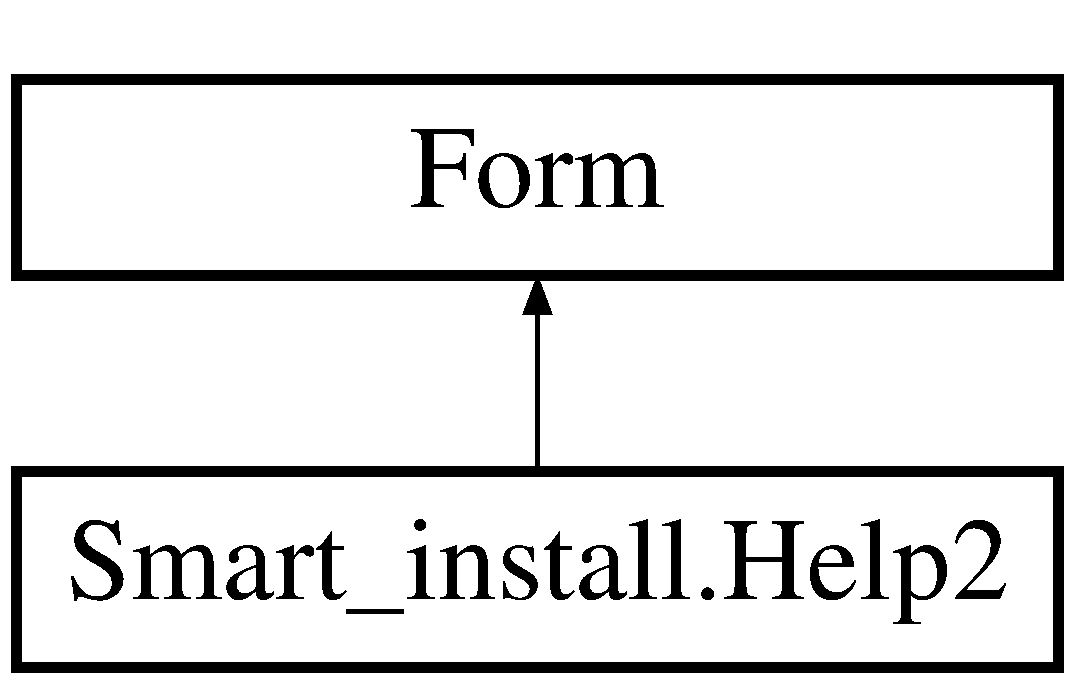
\includegraphics[height=2.000000cm]{class_smart__install_1_1_help2}
\end{center}
\end{figure}
\subsection*{Metody publiczne}
\begin{DoxyCompactItemize}
\item 
\hyperlink{class_smart__install_1_1_help2_a8abd69b15fa766c2bfe0e459cfcbc864}{Help2} ()
\end{DoxyCompactItemize}
\subsection*{Metody chronione}
\begin{DoxyCompactItemize}
\item 
override void \hyperlink{class_smart__install_1_1_help2_a43eab4ead68724b6d3d63290d534cdb5}{Dispose} (bool disposing)
\begin{DoxyCompactList}\small\item\em Clean up any resources being used. \end{DoxyCompactList}\end{DoxyCompactItemize}


\subsection{Opis szczegółowy}


Definicja w linii 13 pliku Help2.\+cs.



\subsection{Dokumentacja konstruktora i destruktora}
\hypertarget{class_smart__install_1_1_help2_a8abd69b15fa766c2bfe0e459cfcbc864}{\index{Smart\+\_\+install\+::\+Help2@{Smart\+\_\+install\+::\+Help2}!Help2@{Help2}}
\index{Help2@{Help2}!Smart\+\_\+install\+::\+Help2@{Smart\+\_\+install\+::\+Help2}}
\subsubsection[{Help2}]{\setlength{\rightskip}{0pt plus 5cm}Smart\+\_\+install.\+Help2.\+Help2 (
\begin{DoxyParamCaption}
{}
\end{DoxyParamCaption}
)}}\label{class_smart__install_1_1_help2_a8abd69b15fa766c2bfe0e459cfcbc864}


Definicja w linii 15 pliku Help2.\+cs.



\subsection{Dokumentacja funkcji składowych}
\hypertarget{class_smart__install_1_1_help2_a43eab4ead68724b6d3d63290d534cdb5}{\index{Smart\+\_\+install\+::\+Help2@{Smart\+\_\+install\+::\+Help2}!Dispose@{Dispose}}
\index{Dispose@{Dispose}!Smart\+\_\+install\+::\+Help2@{Smart\+\_\+install\+::\+Help2}}
\subsubsection[{Dispose}]{\setlength{\rightskip}{0pt plus 5cm}override void Smart\+\_\+install.\+Help2.\+Dispose (
\begin{DoxyParamCaption}
\item[{bool}]{disposing}
\end{DoxyParamCaption}
)\hspace{0.3cm}{\ttfamily [protected]}}}\label{class_smart__install_1_1_help2_a43eab4ead68724b6d3d63290d534cdb5}


Clean up any resources being used. 


\begin{DoxyParams}{Parametry}
{\em disposing} & true if managed resources should be disposed; otherwise, false.\\
\hline
\end{DoxyParams}


Definicja w linii 14 pliku Help2.\+Designer.\+cs.



Dokumentacja dla tej klasy została wygenerowana z plików\+:\begin{DoxyCompactItemize}
\item 
\hyperlink{_help2_8cs}{Help2.\+cs}\item 
\hyperlink{_help2_8_designer_8cs}{Help2.\+Designer.\+cs}\end{DoxyCompactItemize}

\hypertarget{struct_smart__install_1_1_search_program_1_1_install_program}{\section{Dokumentacja struktury Smart\+\_\+install.\+Search\+Program.\+Install\+Program}
\label{struct_smart__install_1_1_search_program_1_1_install_program}\index{Smart\+\_\+install.\+Search\+Program.\+Install\+Program@{Smart\+\_\+install.\+Search\+Program.\+Install\+Program}}
}
\subsection*{Atrybuty publiczne}
\begin{DoxyCompactItemize}
\item 
string \hyperlink{struct_smart__install_1_1_search_program_1_1_install_program_a07c41cefb50c426c1df814338c30a478}{display\+Name}
\item 
string \hyperlink{struct_smart__install_1_1_search_program_1_1_install_program_ae0e1bf0c9bae9086be9174f97da9884f}{display\+Version}
\item 
string \hyperlink{struct_smart__install_1_1_search_program_1_1_install_program_a4328e53b176bc95dbeeda397045f893b}{comments}
\item 
string \hyperlink{struct_smart__install_1_1_search_program_1_1_install_program_a9ac05784dcc59e1f79fe162c873d48d7}{contact}
\item 
string \hyperlink{struct_smart__install_1_1_search_program_1_1_install_program_a343596c9b762754aa6875d7241a2f331}{help\+Link}
\item 
string \hyperlink{struct_smart__install_1_1_search_program_1_1_install_program_a3088b7eee1a31636eb1f874087f13644}{install\+Date}
\item 
string \hyperlink{struct_smart__install_1_1_search_program_1_1_install_program_aaf8fac1b00267733b9b77b05eeea0cf8}{install\+Location}
\item 
string \hyperlink{struct_smart__install_1_1_search_program_1_1_install_program_a8934b1419bdba4c690faec433c722d81}{language}
\item 
string \hyperlink{struct_smart__install_1_1_search_program_1_1_install_program_ac037e0544c982fbda344ce0fb8af4062}{modify\+Path}
\end{DoxyCompactItemize}


\subsection{Opis szczegółowy}


Definicja w linii 14 pliku Search\+Program.\+cs.



\subsection{Dokumentacja atrybutów składowych}
\hypertarget{struct_smart__install_1_1_search_program_1_1_install_program_a4328e53b176bc95dbeeda397045f893b}{\index{Smart\+\_\+install\+::\+Search\+Program\+::\+Install\+Program@{Smart\+\_\+install\+::\+Search\+Program\+::\+Install\+Program}!comments@{comments}}
\index{comments@{comments}!Smart\+\_\+install\+::\+Search\+Program\+::\+Install\+Program@{Smart\+\_\+install\+::\+Search\+Program\+::\+Install\+Program}}
\subsubsection[{comments}]{\setlength{\rightskip}{0pt plus 5cm}string Smart\+\_\+install.\+Search\+Program.\+Install\+Program.\+comments}}\label{struct_smart__install_1_1_search_program_1_1_install_program_a4328e53b176bc95dbeeda397045f893b}


Definicja w linii 18 pliku Search\+Program.\+cs.

\hypertarget{struct_smart__install_1_1_search_program_1_1_install_program_a9ac05784dcc59e1f79fe162c873d48d7}{\index{Smart\+\_\+install\+::\+Search\+Program\+::\+Install\+Program@{Smart\+\_\+install\+::\+Search\+Program\+::\+Install\+Program}!contact@{contact}}
\index{contact@{contact}!Smart\+\_\+install\+::\+Search\+Program\+::\+Install\+Program@{Smart\+\_\+install\+::\+Search\+Program\+::\+Install\+Program}}
\subsubsection[{contact}]{\setlength{\rightskip}{0pt plus 5cm}string Smart\+\_\+install.\+Search\+Program.\+Install\+Program.\+contact}}\label{struct_smart__install_1_1_search_program_1_1_install_program_a9ac05784dcc59e1f79fe162c873d48d7}


Definicja w linii 19 pliku Search\+Program.\+cs.

\hypertarget{struct_smart__install_1_1_search_program_1_1_install_program_a07c41cefb50c426c1df814338c30a478}{\index{Smart\+\_\+install\+::\+Search\+Program\+::\+Install\+Program@{Smart\+\_\+install\+::\+Search\+Program\+::\+Install\+Program}!display\+Name@{display\+Name}}
\index{display\+Name@{display\+Name}!Smart\+\_\+install\+::\+Search\+Program\+::\+Install\+Program@{Smart\+\_\+install\+::\+Search\+Program\+::\+Install\+Program}}
\subsubsection[{display\+Name}]{\setlength{\rightskip}{0pt plus 5cm}string Smart\+\_\+install.\+Search\+Program.\+Install\+Program.\+display\+Name}}\label{struct_smart__install_1_1_search_program_1_1_install_program_a07c41cefb50c426c1df814338c30a478}


Definicja w linii 16 pliku Search\+Program.\+cs.

\hypertarget{struct_smart__install_1_1_search_program_1_1_install_program_ae0e1bf0c9bae9086be9174f97da9884f}{\index{Smart\+\_\+install\+::\+Search\+Program\+::\+Install\+Program@{Smart\+\_\+install\+::\+Search\+Program\+::\+Install\+Program}!display\+Version@{display\+Version}}
\index{display\+Version@{display\+Version}!Smart\+\_\+install\+::\+Search\+Program\+::\+Install\+Program@{Smart\+\_\+install\+::\+Search\+Program\+::\+Install\+Program}}
\subsubsection[{display\+Version}]{\setlength{\rightskip}{0pt plus 5cm}string Smart\+\_\+install.\+Search\+Program.\+Install\+Program.\+display\+Version}}\label{struct_smart__install_1_1_search_program_1_1_install_program_ae0e1bf0c9bae9086be9174f97da9884f}


Definicja w linii 17 pliku Search\+Program.\+cs.

\hypertarget{struct_smart__install_1_1_search_program_1_1_install_program_a343596c9b762754aa6875d7241a2f331}{\index{Smart\+\_\+install\+::\+Search\+Program\+::\+Install\+Program@{Smart\+\_\+install\+::\+Search\+Program\+::\+Install\+Program}!help\+Link@{help\+Link}}
\index{help\+Link@{help\+Link}!Smart\+\_\+install\+::\+Search\+Program\+::\+Install\+Program@{Smart\+\_\+install\+::\+Search\+Program\+::\+Install\+Program}}
\subsubsection[{help\+Link}]{\setlength{\rightskip}{0pt plus 5cm}string Smart\+\_\+install.\+Search\+Program.\+Install\+Program.\+help\+Link}}\label{struct_smart__install_1_1_search_program_1_1_install_program_a343596c9b762754aa6875d7241a2f331}


Definicja w linii 20 pliku Search\+Program.\+cs.

\hypertarget{struct_smart__install_1_1_search_program_1_1_install_program_a3088b7eee1a31636eb1f874087f13644}{\index{Smart\+\_\+install\+::\+Search\+Program\+::\+Install\+Program@{Smart\+\_\+install\+::\+Search\+Program\+::\+Install\+Program}!install\+Date@{install\+Date}}
\index{install\+Date@{install\+Date}!Smart\+\_\+install\+::\+Search\+Program\+::\+Install\+Program@{Smart\+\_\+install\+::\+Search\+Program\+::\+Install\+Program}}
\subsubsection[{install\+Date}]{\setlength{\rightskip}{0pt plus 5cm}string Smart\+\_\+install.\+Search\+Program.\+Install\+Program.\+install\+Date}}\label{struct_smart__install_1_1_search_program_1_1_install_program_a3088b7eee1a31636eb1f874087f13644}


Definicja w linii 21 pliku Search\+Program.\+cs.

\hypertarget{struct_smart__install_1_1_search_program_1_1_install_program_aaf8fac1b00267733b9b77b05eeea0cf8}{\index{Smart\+\_\+install\+::\+Search\+Program\+::\+Install\+Program@{Smart\+\_\+install\+::\+Search\+Program\+::\+Install\+Program}!install\+Location@{install\+Location}}
\index{install\+Location@{install\+Location}!Smart\+\_\+install\+::\+Search\+Program\+::\+Install\+Program@{Smart\+\_\+install\+::\+Search\+Program\+::\+Install\+Program}}
\subsubsection[{install\+Location}]{\setlength{\rightskip}{0pt plus 5cm}string Smart\+\_\+install.\+Search\+Program.\+Install\+Program.\+install\+Location}}\label{struct_smart__install_1_1_search_program_1_1_install_program_aaf8fac1b00267733b9b77b05eeea0cf8}


Definicja w linii 22 pliku Search\+Program.\+cs.

\hypertarget{struct_smart__install_1_1_search_program_1_1_install_program_a8934b1419bdba4c690faec433c722d81}{\index{Smart\+\_\+install\+::\+Search\+Program\+::\+Install\+Program@{Smart\+\_\+install\+::\+Search\+Program\+::\+Install\+Program}!language@{language}}
\index{language@{language}!Smart\+\_\+install\+::\+Search\+Program\+::\+Install\+Program@{Smart\+\_\+install\+::\+Search\+Program\+::\+Install\+Program}}
\subsubsection[{language}]{\setlength{\rightskip}{0pt plus 5cm}string Smart\+\_\+install.\+Search\+Program.\+Install\+Program.\+language}}\label{struct_smart__install_1_1_search_program_1_1_install_program_a8934b1419bdba4c690faec433c722d81}


Definicja w linii 23 pliku Search\+Program.\+cs.

\hypertarget{struct_smart__install_1_1_search_program_1_1_install_program_ac037e0544c982fbda344ce0fb8af4062}{\index{Smart\+\_\+install\+::\+Search\+Program\+::\+Install\+Program@{Smart\+\_\+install\+::\+Search\+Program\+::\+Install\+Program}!modify\+Path@{modify\+Path}}
\index{modify\+Path@{modify\+Path}!Smart\+\_\+install\+::\+Search\+Program\+::\+Install\+Program@{Smart\+\_\+install\+::\+Search\+Program\+::\+Install\+Program}}
\subsubsection[{modify\+Path}]{\setlength{\rightskip}{0pt plus 5cm}string Smart\+\_\+install.\+Search\+Program.\+Install\+Program.\+modify\+Path}}\label{struct_smart__install_1_1_search_program_1_1_install_program_ac037e0544c982fbda344ce0fb8af4062}


Definicja w linii 24 pliku Search\+Program.\+cs.



Dokumentacja dla tej struktury została wygenerowana z pliku\+:\begin{DoxyCompactItemize}
\item 
\hyperlink{_search_program_8cs}{Search\+Program.\+cs}\end{DoxyCompactItemize}

\hypertarget{class_smart__install_1_1_language}{\section{Dokumentacja klasy Smart\+\_\+install.\+Language}
\label{class_smart__install_1_1_language}\index{Smart\+\_\+install.\+Language@{Smart\+\_\+install.\+Language}}
}
\subsection*{Metody publiczne}
\begin{DoxyCompactItemize}
\item 
\hyperlink{class_smart__install_1_1_language_ac9bbdf77724f397f58954c9c3e75cf03}{Language} ()
\end{DoxyCompactItemize}
\subsection*{Właściwości}
\begin{DoxyCompactItemize}
\item 
int \hyperlink{class_smart__install_1_1_language_a38247b2fb0320ba0e0a70efab8927dd3}{Id}\hspace{0.3cm}{\ttfamily  \mbox{[}get, set\mbox{]}}
\item 
string \hyperlink{class_smart__install_1_1_language_a49c0c02bcda046b771c222941569927a}{Language1}\hspace{0.3cm}{\ttfamily  \mbox{[}get, set\mbox{]}}
\item 
virtual I\+Collection$<$ \hyperlink{class_smart__install_1_1_prog}{Prog} $>$ \hyperlink{class_smart__install_1_1_language_a23f806e2c30c3b9eae478ad27fc53123}{Progs}\hspace{0.3cm}{\ttfamily  \mbox{[}get, set\mbox{]}}
\end{DoxyCompactItemize}


\subsection{Opis szczegółowy}


Definicja w linii 15 pliku Language.\+cs.



\subsection{Dokumentacja konstruktora i destruktora}
\hypertarget{class_smart__install_1_1_language_ac9bbdf77724f397f58954c9c3e75cf03}{\index{Smart\+\_\+install\+::\+Language@{Smart\+\_\+install\+::\+Language}!Language@{Language}}
\index{Language@{Language}!Smart\+\_\+install\+::\+Language@{Smart\+\_\+install\+::\+Language}}
\subsubsection[{Language}]{\setlength{\rightskip}{0pt plus 5cm}Smart\+\_\+install.\+Language.\+Language (
\begin{DoxyParamCaption}
{}
\end{DoxyParamCaption}
)}}\label{class_smart__install_1_1_language_ac9bbdf77724f397f58954c9c3e75cf03}


Definicja w linii 17 pliku Language.\+cs.



\subsection{Dokumentacja właściwości}
\hypertarget{class_smart__install_1_1_language_a38247b2fb0320ba0e0a70efab8927dd3}{\index{Smart\+\_\+install\+::\+Language@{Smart\+\_\+install\+::\+Language}!Id@{Id}}
\index{Id@{Id}!Smart\+\_\+install\+::\+Language@{Smart\+\_\+install\+::\+Language}}
\subsubsection[{Id}]{\setlength{\rightskip}{0pt plus 5cm}int Smart\+\_\+install.\+Language.\+Id\hspace{0.3cm}{\ttfamily [get]}, {\ttfamily [set]}}}\label{class_smart__install_1_1_language_a38247b2fb0320ba0e0a70efab8927dd3}


Definicja w linii 22 pliku Language.\+cs.

\hypertarget{class_smart__install_1_1_language_a49c0c02bcda046b771c222941569927a}{\index{Smart\+\_\+install\+::\+Language@{Smart\+\_\+install\+::\+Language}!Language1@{Language1}}
\index{Language1@{Language1}!Smart\+\_\+install\+::\+Language@{Smart\+\_\+install\+::\+Language}}
\subsubsection[{Language1}]{\setlength{\rightskip}{0pt plus 5cm}string Smart\+\_\+install.\+Language.\+Language1\hspace{0.3cm}{\ttfamily [get]}, {\ttfamily [set]}}}\label{class_smart__install_1_1_language_a49c0c02bcda046b771c222941569927a}


Definicja w linii 23 pliku Language.\+cs.

\hypertarget{class_smart__install_1_1_language_a23f806e2c30c3b9eae478ad27fc53123}{\index{Smart\+\_\+install\+::\+Language@{Smart\+\_\+install\+::\+Language}!Progs@{Progs}}
\index{Progs@{Progs}!Smart\+\_\+install\+::\+Language@{Smart\+\_\+install\+::\+Language}}
\subsubsection[{Progs}]{\setlength{\rightskip}{0pt plus 5cm}virtual I\+Collection$<${\bf Prog}$>$ Smart\+\_\+install.\+Language.\+Progs\hspace{0.3cm}{\ttfamily [get]}, {\ttfamily [set]}}}\label{class_smart__install_1_1_language_a23f806e2c30c3b9eae478ad27fc53123}


Definicja w linii 25 pliku Language.\+cs.



Dokumentacja dla tej klasy została wygenerowana z pliku\+:\begin{DoxyCompactItemize}
\item 
\hyperlink{_language_8cs}{Language.\+cs}\end{DoxyCompactItemize}

\hypertarget{class_smart__install_1_1_menu_install}{\section{Dokumentacja klasy Smart\+\_\+install.\+Menu\+Install}
\label{class_smart__install_1_1_menu_install}\index{Smart\+\_\+install.\+Menu\+Install@{Smart\+\_\+install.\+Menu\+Install}}
}
Diagram dziedziczenia dla Smart\+\_\+install.\+Menu\+Install\begin{figure}[H]
\begin{center}
\leavevmode
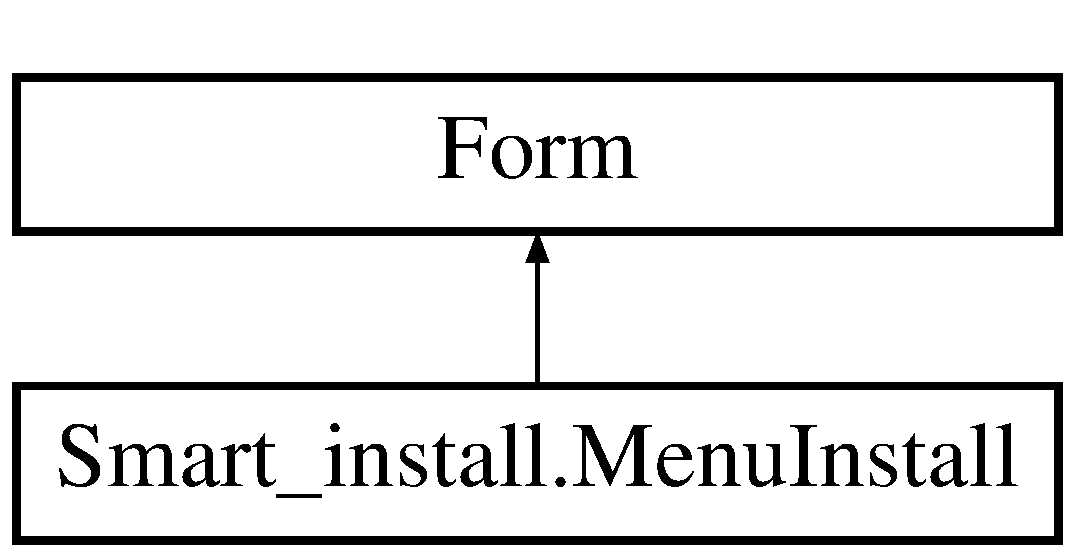
\includegraphics[height=2.000000cm]{class_smart__install_1_1_menu_install}
\end{center}
\end{figure}
\subsection*{Metody publiczne}
\begin{DoxyCompactItemize}
\item 
\hyperlink{class_smart__install_1_1_menu_install_a33c8f9d55d877fd5c471dae0f0d6d4dd}{Menu\+Install} (List$<$ \hyperlink{class_smart__install_1_1program_information}{program\+Information} $>$ progs)
\end{DoxyCompactItemize}
\subsection*{Metody chronione}
\begin{DoxyCompactItemize}
\item 
override void \hyperlink{class_smart__install_1_1_menu_install_af0e1e2239a2c2c3aa39a2ec98e9d302c}{Dispose} (bool disposing)
\begin{DoxyCompactList}\small\item\em Clean up any resources being used. \end{DoxyCompactList}\end{DoxyCompactItemize}


\subsection{Opis szczegółowy}


Definicja w linii 13 pliku Menu\+Install.\+cs.



\subsection{Dokumentacja konstruktora i destruktora}
\hypertarget{class_smart__install_1_1_menu_install_a33c8f9d55d877fd5c471dae0f0d6d4dd}{\index{Smart\+\_\+install\+::\+Menu\+Install@{Smart\+\_\+install\+::\+Menu\+Install}!Menu\+Install@{Menu\+Install}}
\index{Menu\+Install@{Menu\+Install}!Smart\+\_\+install\+::\+Menu\+Install@{Smart\+\_\+install\+::\+Menu\+Install}}
\subsubsection[{Menu\+Install}]{\setlength{\rightskip}{0pt plus 5cm}Smart\+\_\+install.\+Menu\+Install.\+Menu\+Install (
\begin{DoxyParamCaption}
\item[{List$<$ {\bf program\+Information} $>$}]{progs}
\end{DoxyParamCaption}
)}}\label{class_smart__install_1_1_menu_install_a33c8f9d55d877fd5c471dae0f0d6d4dd}


Definicja w linii 16 pliku Menu\+Install.\+cs.



\subsection{Dokumentacja funkcji składowych}
\hypertarget{class_smart__install_1_1_menu_install_af0e1e2239a2c2c3aa39a2ec98e9d302c}{\index{Smart\+\_\+install\+::\+Menu\+Install@{Smart\+\_\+install\+::\+Menu\+Install}!Dispose@{Dispose}}
\index{Dispose@{Dispose}!Smart\+\_\+install\+::\+Menu\+Install@{Smart\+\_\+install\+::\+Menu\+Install}}
\subsubsection[{Dispose}]{\setlength{\rightskip}{0pt plus 5cm}override void Smart\+\_\+install.\+Menu\+Install.\+Dispose (
\begin{DoxyParamCaption}
\item[{bool}]{disposing}
\end{DoxyParamCaption}
)\hspace{0.3cm}{\ttfamily [protected]}}}\label{class_smart__install_1_1_menu_install_af0e1e2239a2c2c3aa39a2ec98e9d302c}


Clean up any resources being used. 


\begin{DoxyParams}{Parametry}
{\em disposing} & true if managed resources should be disposed; otherwise, false.\\
\hline
\end{DoxyParams}


Definicja w linii 14 pliku Menu\+Install.\+Designer.\+cs.



Dokumentacja dla tej klasy została wygenerowana z plików\+:\begin{DoxyCompactItemize}
\item 
\hyperlink{_menu_install_8cs}{Menu\+Install.\+cs}\item 
\hyperlink{_menu_install_8_designer_8cs}{Menu\+Install.\+Designer.\+cs}\end{DoxyCompactItemize}

\hypertarget{class_smart__install_1_1_new_arch}{\section{Dokumentacja klasy Smart\+\_\+install.\+New\+Arch}
\label{class_smart__install_1_1_new_arch}\index{Smart\+\_\+install.\+New\+Arch@{Smart\+\_\+install.\+New\+Arch}}
}
Diagram dziedziczenia dla Smart\+\_\+install.\+New\+Arch\begin{figure}[H]
\begin{center}
\leavevmode
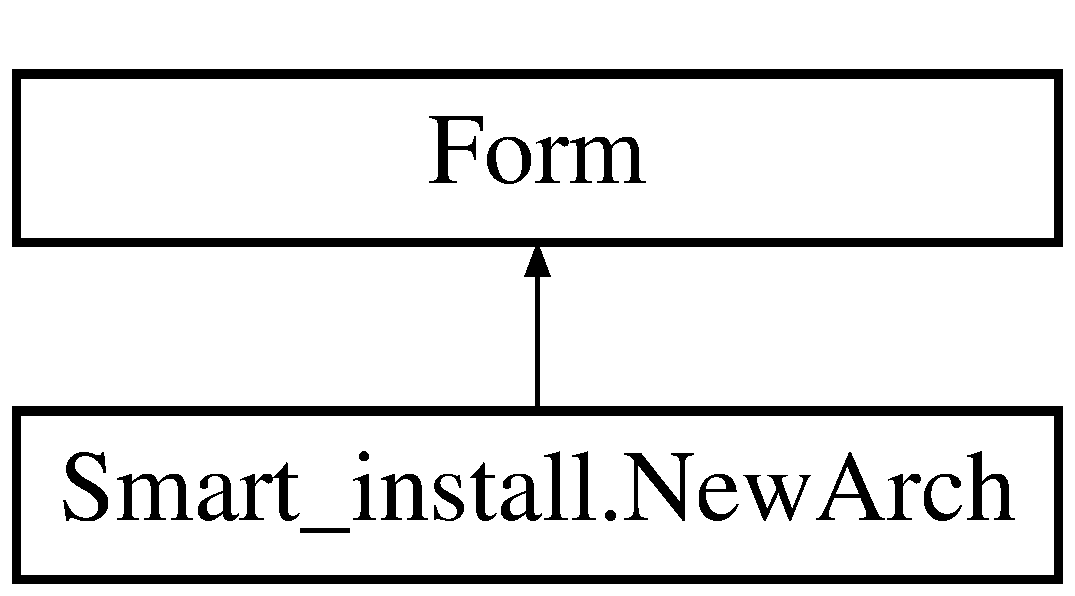
\includegraphics[height=2.000000cm]{class_smart__install_1_1_new_arch}
\end{center}
\end{figure}
\subsection*{Metody publiczne}
\begin{DoxyCompactItemize}
\item 
\hyperlink{class_smart__install_1_1_new_arch_aa9169659caa4fa4e2a273d8dc6076362}{New\+Arch} (\hyperlink{class_smart__install_1_1user_menu_install}{user\+Menu\+Install} parent)
\item 
void \hyperlink{class_smart__install_1_1_new_arch_a73f1f94a96c3e3a0c3729673aeb2caa8}{refresh} ()
\begin{DoxyCompactList}\small\item\em sprawdzam czy zostało zaznaczony jakis tak , jeśli tak to dodaje go do \+\_\+selecttag a w przeciwnym wypadku to usuwam go z \+\_\+selecttag zapyta o programy z tagow (string) \end{DoxyCompactList}\item 
void \hyperlink{class_smart__install_1_1_new_arch_a7d8c334fdfb9872ce29ac88d9d8fbd8f}{add\+Program} (\hyperlink{class_smart__install_1_1program_information}{program\+Information} prog, string tag=null)
\item 
void \hyperlink{class_smart__install_1_1_new_arch_a5dc5c16b7ae357601c701f0d90819000}{Delete\+Program} (string p)
\end{DoxyCompactItemize}
\subsection*{Metody chronione}
\begin{DoxyCompactItemize}
\item 
override void \hyperlink{class_smart__install_1_1_new_arch_ae0b2866651d46def93594aa2665b876d}{Dispose} (bool disposing)
\begin{DoxyCompactList}\small\item\em Clean up any resources being used. \end{DoxyCompactList}\end{DoxyCompactItemize}
\subsection*{Właściwości}
\begin{DoxyCompactItemize}
\item 
List$<$ \hyperlink{class_smart__install_1_1program_information}{program\+Information} $>$ \hyperlink{class_smart__install_1_1_new_arch_a614a85108ae7c4362e3f813a1349c372}{all\+Programs}\hspace{0.3cm}{\ttfamily  \mbox{[}get\mbox{]}}
\end{DoxyCompactItemize}


\subsection{Opis szczegółowy}


Definicja w linii 15 pliku New\+Arch.\+cs.



\subsection{Dokumentacja konstruktora i destruktora}
\hypertarget{class_smart__install_1_1_new_arch_aa9169659caa4fa4e2a273d8dc6076362}{\index{Smart\+\_\+install\+::\+New\+Arch@{Smart\+\_\+install\+::\+New\+Arch}!New\+Arch@{New\+Arch}}
\index{New\+Arch@{New\+Arch}!Smart\+\_\+install\+::\+New\+Arch@{Smart\+\_\+install\+::\+New\+Arch}}
\subsubsection[{New\+Arch}]{\setlength{\rightskip}{0pt plus 5cm}Smart\+\_\+install.\+New\+Arch.\+New\+Arch (
\begin{DoxyParamCaption}
\item[{{\bf user\+Menu\+Install}}]{parent}
\end{DoxyParamCaption}
)}}\label{class_smart__install_1_1_new_arch_aa9169659caa4fa4e2a273d8dc6076362}


Definicja w linii 30 pliku New\+Arch.\+cs.



\subsection{Dokumentacja funkcji składowych}
\hypertarget{class_smart__install_1_1_new_arch_a7d8c334fdfb9872ce29ac88d9d8fbd8f}{\index{Smart\+\_\+install\+::\+New\+Arch@{Smart\+\_\+install\+::\+New\+Arch}!add\+Program@{add\+Program}}
\index{add\+Program@{add\+Program}!Smart\+\_\+install\+::\+New\+Arch@{Smart\+\_\+install\+::\+New\+Arch}}
\subsubsection[{add\+Program}]{\setlength{\rightskip}{0pt plus 5cm}void Smart\+\_\+install.\+New\+Arch.\+add\+Program (
\begin{DoxyParamCaption}
\item[{{\bf program\+Information}}]{prog, }
\item[{string}]{tag = {\ttfamily null}}
\end{DoxyParamCaption}
)}}\label{class_smart__install_1_1_new_arch_a7d8c334fdfb9872ce29ac88d9d8fbd8f}


Definicja w linii 117 pliku New\+Arch.\+cs.

\hypertarget{class_smart__install_1_1_new_arch_a5dc5c16b7ae357601c701f0d90819000}{\index{Smart\+\_\+install\+::\+New\+Arch@{Smart\+\_\+install\+::\+New\+Arch}!Delete\+Program@{Delete\+Program}}
\index{Delete\+Program@{Delete\+Program}!Smart\+\_\+install\+::\+New\+Arch@{Smart\+\_\+install\+::\+New\+Arch}}
\subsubsection[{Delete\+Program}]{\setlength{\rightskip}{0pt plus 5cm}void Smart\+\_\+install.\+New\+Arch.\+Delete\+Program (
\begin{DoxyParamCaption}
\item[{string}]{p}
\end{DoxyParamCaption}
)}}\label{class_smart__install_1_1_new_arch_a5dc5c16b7ae357601c701f0d90819000}


Definicja w linii 361 pliku New\+Arch.\+cs.

\hypertarget{class_smart__install_1_1_new_arch_ae0b2866651d46def93594aa2665b876d}{\index{Smart\+\_\+install\+::\+New\+Arch@{Smart\+\_\+install\+::\+New\+Arch}!Dispose@{Dispose}}
\index{Dispose@{Dispose}!Smart\+\_\+install\+::\+New\+Arch@{Smart\+\_\+install\+::\+New\+Arch}}
\subsubsection[{Dispose}]{\setlength{\rightskip}{0pt plus 5cm}override void Smart\+\_\+install.\+New\+Arch.\+Dispose (
\begin{DoxyParamCaption}
\item[{bool}]{disposing}
\end{DoxyParamCaption}
)\hspace{0.3cm}{\ttfamily [protected]}}}\label{class_smart__install_1_1_new_arch_ae0b2866651d46def93594aa2665b876d}


Clean up any resources being used. 


\begin{DoxyParams}{Parametry}
{\em disposing} & true if managed resources should be disposed; otherwise, false.\\
\hline
\end{DoxyParams}


Definicja w linii 14 pliku New\+Arch.\+Designer.\+cs.

\hypertarget{class_smart__install_1_1_new_arch_a73f1f94a96c3e3a0c3729673aeb2caa8}{\index{Smart\+\_\+install\+::\+New\+Arch@{Smart\+\_\+install\+::\+New\+Arch}!refresh@{refresh}}
\index{refresh@{refresh}!Smart\+\_\+install\+::\+New\+Arch@{Smart\+\_\+install\+::\+New\+Arch}}
\subsubsection[{refresh}]{\setlength{\rightskip}{0pt plus 5cm}void Smart\+\_\+install.\+New\+Arch.\+refresh (
\begin{DoxyParamCaption}
{}
\end{DoxyParamCaption}
)}}\label{class_smart__install_1_1_new_arch_a73f1f94a96c3e3a0c3729673aeb2caa8}


sprawdzam czy zostało zaznaczony jakis tak , jeśli tak to dodaje go do \+\_\+selecttag a w przeciwnym wypadku to usuwam go z \+\_\+selecttag zapyta o programy z tagow (string) 


\begin{DoxyParams}{Parametry}
{\em sender} & \\
\hline
{\em e} & \\
\hline
\end{DoxyParams}


Definicja w linii 98 pliku New\+Arch.\+cs.



\subsection{Dokumentacja właściwości}
\hypertarget{class_smart__install_1_1_new_arch_a614a85108ae7c4362e3f813a1349c372}{\index{Smart\+\_\+install\+::\+New\+Arch@{Smart\+\_\+install\+::\+New\+Arch}!all\+Programs@{all\+Programs}}
\index{all\+Programs@{all\+Programs}!Smart\+\_\+install\+::\+New\+Arch@{Smart\+\_\+install\+::\+New\+Arch}}
\subsubsection[{all\+Programs}]{\setlength{\rightskip}{0pt plus 5cm}List$<${\bf program\+Information}$>$ Smart\+\_\+install.\+New\+Arch.\+all\+Programs\hspace{0.3cm}{\ttfamily [get]}}}\label{class_smart__install_1_1_new_arch_a614a85108ae7c4362e3f813a1349c372}


Definicja w linii 23 pliku New\+Arch.\+cs.



Dokumentacja dla tej klasy została wygenerowana z plików\+:\begin{DoxyCompactItemize}
\item 
\hyperlink{_new_arch_8cs}{New\+Arch.\+cs}\item 
\hyperlink{_new_arch_8_designer_8cs}{New\+Arch.\+Designer.\+cs}\end{DoxyCompactItemize}

\hypertarget{class_smart__install_1_1_prog}{\section{Dokumentacja klasy Smart\+\_\+install.\+Prog}
\label{class_smart__install_1_1_prog}\index{Smart\+\_\+install.\+Prog@{Smart\+\_\+install.\+Prog}}
}
\subsection*{Metody publiczne}
\begin{DoxyCompactItemize}
\item 
\hyperlink{class_smart__install_1_1_prog_afb48dfb11267b4c035de65967a88d0b6}{Prog} ()
\end{DoxyCompactItemize}
\subsection*{Właściwości}
\begin{DoxyCompactItemize}
\item 
int \hyperlink{class_smart__install_1_1_prog_aa2d0ae5b2e90aed283c33d2c31f2e0ea}{Id}\hspace{0.3cm}{\ttfamily  \mbox{[}get, set\mbox{]}}
\item 
string \hyperlink{class_smart__install_1_1_prog_a27bb79e4d190a1233ea020dd5e42640b}{Name}\hspace{0.3cm}{\ttfamily  \mbox{[}get, set\mbox{]}}
\item 
string \hyperlink{class_smart__install_1_1_prog_afe5824034eb128c9cbf4070662d9bfc5}{Version}\hspace{0.3cm}{\ttfamily  \mbox{[}get, set\mbox{]}}
\item 
string \hyperlink{class_smart__install_1_1_prog_aca24c50cd14e1b94afe4e11ab6473374}{Description}\hspace{0.3cm}{\ttfamily  \mbox{[}get, set\mbox{]}}
\item 
string \hyperlink{class_smart__install_1_1_prog_a01ce20f56b0c1d25333642c479fc0ca8}{Help\+Link}\hspace{0.3cm}{\ttfamily  \mbox{[}get, set\mbox{]}}
\item 
string \hyperlink{class_smart__install_1_1_prog_adbdecfb233f4747de164aa713e0eb9b9}{U\+R\+L\+Update}\hspace{0.3cm}{\ttfamily  \mbox{[}get, set\mbox{]}}
\item 
string \hyperlink{class_smart__install_1_1_prog_a7323e69631bf602cefbdb2e500553ec7}{Publisher}\hspace{0.3cm}{\ttfamily  \mbox{[}get, set\mbox{]}}
\item 
string \hyperlink{class_smart__install_1_1_prog_a897d5c26dbfb350ef8c270f46275122e}{Icon}\hspace{0.3cm}{\ttfamily  \mbox{[}get, set\mbox{]}}
\item 
Nullable$<$ int $>$ \hyperlink{class_smart__install_1_1_prog_a42c854c682c1c2856bb3212930126cb7}{Language\+I\+D}\hspace{0.3cm}{\ttfamily  \mbox{[}get, set\mbox{]}}
\item 
Nullable$<$ int $>$ \hyperlink{class_smart__install_1_1_prog_abba886f20aedba13ab6739e4726eaf22}{System\+I\+D}\hspace{0.3cm}{\ttfamily  \mbox{[}get, set\mbox{]}}
\item 
virtual \hyperlink{class_smart__install_1_1_language}{Language} \hyperlink{class_smart__install_1_1_prog_a74ca35d7e87453b35481b3709ac25605}{Language}\hspace{0.3cm}{\ttfamily  \mbox{[}get, set\mbox{]}}
\item 
virtual \hyperlink{class_smart__install_1_1system_type}{system\+Type} \hyperlink{class_smart__install_1_1_prog_ad590b1e68fbf5df57d8844c8fb438a89}{system\+Type}\hspace{0.3cm}{\ttfamily  \mbox{[}get, set\mbox{]}}
\item 
virtual I\+Collection$<$ \hyperlink{class_smart__install_1_1_archive}{Archive} $>$ \hyperlink{class_smart__install_1_1_prog_a99ebc844dd08ab8e8b3baf64e68067f4}{Archives}\hspace{0.3cm}{\ttfamily  \mbox{[}get, set\mbox{]}}
\item 
virtual I\+Collection$<$ \hyperlink{class_smart__install_1_1_tag}{Tag} $>$ \hyperlink{class_smart__install_1_1_prog_ad3c781481868df3852768412c40490d5}{Tags}\hspace{0.3cm}{\ttfamily  \mbox{[}get, set\mbox{]}}
\end{DoxyCompactItemize}


\subsection{Opis szczegółowy}


Definicja w linii 15 pliku Prog.\+cs.



\subsection{Dokumentacja konstruktora i destruktora}
\hypertarget{class_smart__install_1_1_prog_afb48dfb11267b4c035de65967a88d0b6}{\index{Smart\+\_\+install\+::\+Prog@{Smart\+\_\+install\+::\+Prog}!Prog@{Prog}}
\index{Prog@{Prog}!Smart\+\_\+install\+::\+Prog@{Smart\+\_\+install\+::\+Prog}}
\subsubsection[{Prog}]{\setlength{\rightskip}{0pt plus 5cm}Smart\+\_\+install.\+Prog.\+Prog (
\begin{DoxyParamCaption}
{}
\end{DoxyParamCaption}
)}}\label{class_smart__install_1_1_prog_afb48dfb11267b4c035de65967a88d0b6}


Definicja w linii 17 pliku Prog.\+cs.



\subsection{Dokumentacja właściwości}
\hypertarget{class_smart__install_1_1_prog_a99ebc844dd08ab8e8b3baf64e68067f4}{\index{Smart\+\_\+install\+::\+Prog@{Smart\+\_\+install\+::\+Prog}!Archives@{Archives}}
\index{Archives@{Archives}!Smart\+\_\+install\+::\+Prog@{Smart\+\_\+install\+::\+Prog}}
\subsubsection[{Archives}]{\setlength{\rightskip}{0pt plus 5cm}virtual I\+Collection$<${\bf Archive}$>$ Smart\+\_\+install.\+Prog.\+Archives\hspace{0.3cm}{\ttfamily [get]}, {\ttfamily [set]}}}\label{class_smart__install_1_1_prog_a99ebc844dd08ab8e8b3baf64e68067f4}


Definicja w linii 36 pliku Prog.\+cs.

\hypertarget{class_smart__install_1_1_prog_aca24c50cd14e1b94afe4e11ab6473374}{\index{Smart\+\_\+install\+::\+Prog@{Smart\+\_\+install\+::\+Prog}!Description@{Description}}
\index{Description@{Description}!Smart\+\_\+install\+::\+Prog@{Smart\+\_\+install\+::\+Prog}}
\subsubsection[{Description}]{\setlength{\rightskip}{0pt plus 5cm}string Smart\+\_\+install.\+Prog.\+Description\hspace{0.3cm}{\ttfamily [get]}, {\ttfamily [set]}}}\label{class_smart__install_1_1_prog_aca24c50cd14e1b94afe4e11ab6473374}


Definicja w linii 26 pliku Prog.\+cs.

\hypertarget{class_smart__install_1_1_prog_a01ce20f56b0c1d25333642c479fc0ca8}{\index{Smart\+\_\+install\+::\+Prog@{Smart\+\_\+install\+::\+Prog}!Help\+Link@{Help\+Link}}
\index{Help\+Link@{Help\+Link}!Smart\+\_\+install\+::\+Prog@{Smart\+\_\+install\+::\+Prog}}
\subsubsection[{Help\+Link}]{\setlength{\rightskip}{0pt plus 5cm}string Smart\+\_\+install.\+Prog.\+Help\+Link\hspace{0.3cm}{\ttfamily [get]}, {\ttfamily [set]}}}\label{class_smart__install_1_1_prog_a01ce20f56b0c1d25333642c479fc0ca8}


Definicja w linii 27 pliku Prog.\+cs.

\hypertarget{class_smart__install_1_1_prog_a897d5c26dbfb350ef8c270f46275122e}{\index{Smart\+\_\+install\+::\+Prog@{Smart\+\_\+install\+::\+Prog}!Icon@{Icon}}
\index{Icon@{Icon}!Smart\+\_\+install\+::\+Prog@{Smart\+\_\+install\+::\+Prog}}
\subsubsection[{Icon}]{\setlength{\rightskip}{0pt plus 5cm}string Smart\+\_\+install.\+Prog.\+Icon\hspace{0.3cm}{\ttfamily [get]}, {\ttfamily [set]}}}\label{class_smart__install_1_1_prog_a897d5c26dbfb350ef8c270f46275122e}


Definicja w linii 30 pliku Prog.\+cs.

\hypertarget{class_smart__install_1_1_prog_aa2d0ae5b2e90aed283c33d2c31f2e0ea}{\index{Smart\+\_\+install\+::\+Prog@{Smart\+\_\+install\+::\+Prog}!Id@{Id}}
\index{Id@{Id}!Smart\+\_\+install\+::\+Prog@{Smart\+\_\+install\+::\+Prog}}
\subsubsection[{Id}]{\setlength{\rightskip}{0pt plus 5cm}int Smart\+\_\+install.\+Prog.\+Id\hspace{0.3cm}{\ttfamily [get]}, {\ttfamily [set]}}}\label{class_smart__install_1_1_prog_aa2d0ae5b2e90aed283c33d2c31f2e0ea}


Definicja w linii 23 pliku Prog.\+cs.

\hypertarget{class_smart__install_1_1_prog_a74ca35d7e87453b35481b3709ac25605}{\index{Smart\+\_\+install\+::\+Prog@{Smart\+\_\+install\+::\+Prog}!Language@{Language}}
\index{Language@{Language}!Smart\+\_\+install\+::\+Prog@{Smart\+\_\+install\+::\+Prog}}
\subsubsection[{Language}]{\setlength{\rightskip}{0pt plus 5cm}virtual {\bf Language} Smart\+\_\+install.\+Prog.\+Language\hspace{0.3cm}{\ttfamily [get]}, {\ttfamily [set]}}}\label{class_smart__install_1_1_prog_a74ca35d7e87453b35481b3709ac25605}


Definicja w linii 34 pliku Prog.\+cs.

\hypertarget{class_smart__install_1_1_prog_a42c854c682c1c2856bb3212930126cb7}{\index{Smart\+\_\+install\+::\+Prog@{Smart\+\_\+install\+::\+Prog}!Language\+I\+D@{Language\+I\+D}}
\index{Language\+I\+D@{Language\+I\+D}!Smart\+\_\+install\+::\+Prog@{Smart\+\_\+install\+::\+Prog}}
\subsubsection[{Language\+I\+D}]{\setlength{\rightskip}{0pt plus 5cm}Nullable$<$int$>$ Smart\+\_\+install.\+Prog.\+Language\+I\+D\hspace{0.3cm}{\ttfamily [get]}, {\ttfamily [set]}}}\label{class_smart__install_1_1_prog_a42c854c682c1c2856bb3212930126cb7}


Definicja w linii 31 pliku Prog.\+cs.

\hypertarget{class_smart__install_1_1_prog_a27bb79e4d190a1233ea020dd5e42640b}{\index{Smart\+\_\+install\+::\+Prog@{Smart\+\_\+install\+::\+Prog}!Name@{Name}}
\index{Name@{Name}!Smart\+\_\+install\+::\+Prog@{Smart\+\_\+install\+::\+Prog}}
\subsubsection[{Name}]{\setlength{\rightskip}{0pt plus 5cm}string Smart\+\_\+install.\+Prog.\+Name\hspace{0.3cm}{\ttfamily [get]}, {\ttfamily [set]}}}\label{class_smart__install_1_1_prog_a27bb79e4d190a1233ea020dd5e42640b}


Definicja w linii 24 pliku Prog.\+cs.

\hypertarget{class_smart__install_1_1_prog_a7323e69631bf602cefbdb2e500553ec7}{\index{Smart\+\_\+install\+::\+Prog@{Smart\+\_\+install\+::\+Prog}!Publisher@{Publisher}}
\index{Publisher@{Publisher}!Smart\+\_\+install\+::\+Prog@{Smart\+\_\+install\+::\+Prog}}
\subsubsection[{Publisher}]{\setlength{\rightskip}{0pt plus 5cm}string Smart\+\_\+install.\+Prog.\+Publisher\hspace{0.3cm}{\ttfamily [get]}, {\ttfamily [set]}}}\label{class_smart__install_1_1_prog_a7323e69631bf602cefbdb2e500553ec7}


Definicja w linii 29 pliku Prog.\+cs.

\hypertarget{class_smart__install_1_1_prog_abba886f20aedba13ab6739e4726eaf22}{\index{Smart\+\_\+install\+::\+Prog@{Smart\+\_\+install\+::\+Prog}!System\+I\+D@{System\+I\+D}}
\index{System\+I\+D@{System\+I\+D}!Smart\+\_\+install\+::\+Prog@{Smart\+\_\+install\+::\+Prog}}
\subsubsection[{System\+I\+D}]{\setlength{\rightskip}{0pt plus 5cm}Nullable$<$int$>$ Smart\+\_\+install.\+Prog.\+System\+I\+D\hspace{0.3cm}{\ttfamily [get]}, {\ttfamily [set]}}}\label{class_smart__install_1_1_prog_abba886f20aedba13ab6739e4726eaf22}


Definicja w linii 32 pliku Prog.\+cs.

\hypertarget{class_smart__install_1_1_prog_ad590b1e68fbf5df57d8844c8fb438a89}{\index{Smart\+\_\+install\+::\+Prog@{Smart\+\_\+install\+::\+Prog}!system\+Type@{system\+Type}}
\index{system\+Type@{system\+Type}!Smart\+\_\+install\+::\+Prog@{Smart\+\_\+install\+::\+Prog}}
\subsubsection[{system\+Type}]{\setlength{\rightskip}{0pt plus 5cm}virtual {\bf system\+Type} Smart\+\_\+install.\+Prog.\+system\+Type\hspace{0.3cm}{\ttfamily [get]}, {\ttfamily [set]}}}\label{class_smart__install_1_1_prog_ad590b1e68fbf5df57d8844c8fb438a89}


Definicja w linii 35 pliku Prog.\+cs.

\hypertarget{class_smart__install_1_1_prog_ad3c781481868df3852768412c40490d5}{\index{Smart\+\_\+install\+::\+Prog@{Smart\+\_\+install\+::\+Prog}!Tags@{Tags}}
\index{Tags@{Tags}!Smart\+\_\+install\+::\+Prog@{Smart\+\_\+install\+::\+Prog}}
\subsubsection[{Tags}]{\setlength{\rightskip}{0pt plus 5cm}virtual I\+Collection$<${\bf Tag}$>$ Smart\+\_\+install.\+Prog.\+Tags\hspace{0.3cm}{\ttfamily [get]}, {\ttfamily [set]}}}\label{class_smart__install_1_1_prog_ad3c781481868df3852768412c40490d5}


Definicja w linii 37 pliku Prog.\+cs.

\hypertarget{class_smart__install_1_1_prog_adbdecfb233f4747de164aa713e0eb9b9}{\index{Smart\+\_\+install\+::\+Prog@{Smart\+\_\+install\+::\+Prog}!U\+R\+L\+Update@{U\+R\+L\+Update}}
\index{U\+R\+L\+Update@{U\+R\+L\+Update}!Smart\+\_\+install\+::\+Prog@{Smart\+\_\+install\+::\+Prog}}
\subsubsection[{U\+R\+L\+Update}]{\setlength{\rightskip}{0pt plus 5cm}string Smart\+\_\+install.\+Prog.\+U\+R\+L\+Update\hspace{0.3cm}{\ttfamily [get]}, {\ttfamily [set]}}}\label{class_smart__install_1_1_prog_adbdecfb233f4747de164aa713e0eb9b9}


Definicja w linii 28 pliku Prog.\+cs.

\hypertarget{class_smart__install_1_1_prog_afe5824034eb128c9cbf4070662d9bfc5}{\index{Smart\+\_\+install\+::\+Prog@{Smart\+\_\+install\+::\+Prog}!Version@{Version}}
\index{Version@{Version}!Smart\+\_\+install\+::\+Prog@{Smart\+\_\+install\+::\+Prog}}
\subsubsection[{Version}]{\setlength{\rightskip}{0pt plus 5cm}string Smart\+\_\+install.\+Prog.\+Version\hspace{0.3cm}{\ttfamily [get]}, {\ttfamily [set]}}}\label{class_smart__install_1_1_prog_afe5824034eb128c9cbf4070662d9bfc5}


Definicja w linii 25 pliku Prog.\+cs.



Dokumentacja dla tej klasy została wygenerowana z pliku\+:\begin{DoxyCompactItemize}
\item 
\hyperlink{_prog_8cs}{Prog.\+cs}\end{DoxyCompactItemize}

\hypertarget{class_smart__install_1_1program_information}{\section{Dokumentacja klasy Smart\+\_\+install.\+program\+Information}
\label{class_smart__install_1_1program_information}\index{Smart\+\_\+install.\+program\+Information@{Smart\+\_\+install.\+program\+Information}}
}


Klasa reprezentująca informację na temat programu uzyskiwane od użytkownika  


\subsection*{Metody publiczne}
\begin{DoxyCompactItemize}
\item 
\hyperlink{class_smart__install_1_1program_information_a5ebc2c3214f9f4dea2a95a4bed6e5860}{program\+Information} ()
\item 
\hyperlink{class_smart__install_1_1program_information_aee2ee2515e244d0e11f98acb71287a43}{program\+Information} (\hyperlink{class_smart__install_1_1_prog}{Prog} progr)
\item 
X\+Element \hyperlink{class_smart__install_1_1program_information_a0703329b524464a24398de7fb83e5b66}{get\+X\+Element} ()
\item 
override int \hyperlink{class_smart__install_1_1program_information_a64edbdda5c8d1ae7f3727598b1b82431}{Get\+Hash\+Code} ()
\end{DoxyCompactItemize}
\subsection*{Atrybuty publiczne}
\begin{DoxyCompactItemize}
\item 
int \hyperlink{class_smart__install_1_1program_information_a83edf66af382b3a4e9c1bf2dc94965f2}{Id}
\end{DoxyCompactItemize}
\subsection*{Właściwości}
\begin{DoxyCompactItemize}
\item 
bool \hyperlink{class_smart__install_1_1program_information_a1deafe73f1cf16a6cde32027b58ee395}{is\+Checked}\hspace{0.3cm}{\ttfamily  \mbox{[}get, set\mbox{]}}
\item 
string \hyperlink{class_smart__install_1_1program_information_a813c97c4a629f8cc26d55c22473d2249}{Name}\hspace{0.3cm}{\ttfamily  \mbox{[}get, set\mbox{]}}
\item 
string \hyperlink{class_smart__install_1_1program_information_ae42077cb42cef8cd4ef9c43c0d3b0d55}{Version}\hspace{0.3cm}{\ttfamily  \mbox{[}get, set\mbox{]}}
\item 
string \hyperlink{class_smart__install_1_1program_information_a40f33801171766ccc6474b51686b8e7d}{Description}\hspace{0.3cm}{\ttfamily  \mbox{[}get, set\mbox{]}}
\item 
string \hyperlink{class_smart__install_1_1program_information_a9b1b6ba051cd616bed9cb3d22adff76f}{Help\+Link}\hspace{0.3cm}{\ttfamily  \mbox{[}get, set\mbox{]}}
\item 
string \hyperlink{class_smart__install_1_1program_information_aa3cc9e6105e16a5070dd96a54c58fea2}{U\+R\+L\+Update}\hspace{0.3cm}{\ttfamily  \mbox{[}get, set\mbox{]}}
\item 
Bitmap \hyperlink{class_smart__install_1_1program_information_a05501497d8922e8a4cce6d0205eba546}{Icon}\hspace{0.3cm}{\ttfamily  \mbox{[}get, set\mbox{]}}
\item 
string \hyperlink{class_smart__install_1_1program_information_a1dca0f827edc94e849c3e81a6bd48e5d}{Path}\hspace{0.3cm}{\ttfamily  \mbox{[}get, set\mbox{]}}
\item 
string \hyperlink{class_smart__install_1_1program_information_a452ff269c1ae053f78e04000b29250ae}{Language}\hspace{0.3cm}{\ttfamily  \mbox{[}get, set\mbox{]}}
\item 
string \hyperlink{class_smart__install_1_1program_information_a571313df96dc58540427133224b32b72}{system\+Type}\hspace{0.3cm}{\ttfamily  \mbox{[}get, set\mbox{]}}
\item 
List$<$ string $>$ \hyperlink{class_smart__install_1_1program_information_a1d11c7b990ab03a56bec63af32ab2263}{Tags}\hspace{0.3cm}{\ttfamily  \mbox{[}get, set\mbox{]}}
\end{DoxyCompactItemize}


\subsection{Opis szczegółowy}
Klasa reprezentująca informację na temat programu uzyskiwane od użytkownika 



Definicja w linii 27 pliku control.\+cs.



\subsection{Dokumentacja konstruktora i destruktora}
\hypertarget{class_smart__install_1_1program_information_a5ebc2c3214f9f4dea2a95a4bed6e5860}{\index{Smart\+\_\+install\+::program\+Information@{Smart\+\_\+install\+::program\+Information}!program\+Information@{program\+Information}}
\index{program\+Information@{program\+Information}!Smart\+\_\+install\+::program\+Information@{Smart\+\_\+install\+::program\+Information}}
\subsubsection[{program\+Information}]{\setlength{\rightskip}{0pt plus 5cm}Smart\+\_\+install.\+program\+Information.\+program\+Information (
\begin{DoxyParamCaption}
{}
\end{DoxyParamCaption}
)}}\label{class_smart__install_1_1program_information_a5ebc2c3214f9f4dea2a95a4bed6e5860}


Definicja w linii 56 pliku control.\+cs.

\hypertarget{class_smart__install_1_1program_information_aee2ee2515e244d0e11f98acb71287a43}{\index{Smart\+\_\+install\+::program\+Information@{Smart\+\_\+install\+::program\+Information}!program\+Information@{program\+Information}}
\index{program\+Information@{program\+Information}!Smart\+\_\+install\+::program\+Information@{Smart\+\_\+install\+::program\+Information}}
\subsubsection[{program\+Information}]{\setlength{\rightskip}{0pt plus 5cm}Smart\+\_\+install.\+program\+Information.\+program\+Information (
\begin{DoxyParamCaption}
\item[{{\bf Prog}}]{progr}
\end{DoxyParamCaption}
)}}\label{class_smart__install_1_1program_information_aee2ee2515e244d0e11f98acb71287a43}


Definicja w linii 61 pliku control.\+cs.



\subsection{Dokumentacja funkcji składowych}
\hypertarget{class_smart__install_1_1program_information_a64edbdda5c8d1ae7f3727598b1b82431}{\index{Smart\+\_\+install\+::program\+Information@{Smart\+\_\+install\+::program\+Information}!Get\+Hash\+Code@{Get\+Hash\+Code}}
\index{Get\+Hash\+Code@{Get\+Hash\+Code}!Smart\+\_\+install\+::program\+Information@{Smart\+\_\+install\+::program\+Information}}
\subsubsection[{Get\+Hash\+Code}]{\setlength{\rightskip}{0pt plus 5cm}override int Smart\+\_\+install.\+program\+Information.\+Get\+Hash\+Code (
\begin{DoxyParamCaption}
{}
\end{DoxyParamCaption}
)}}\label{class_smart__install_1_1program_information_a64edbdda5c8d1ae7f3727598b1b82431}


Definicja w linii 100 pliku control.\+cs.

\hypertarget{class_smart__install_1_1program_information_a0703329b524464a24398de7fb83e5b66}{\index{Smart\+\_\+install\+::program\+Information@{Smart\+\_\+install\+::program\+Information}!get\+X\+Element@{get\+X\+Element}}
\index{get\+X\+Element@{get\+X\+Element}!Smart\+\_\+install\+::program\+Information@{Smart\+\_\+install\+::program\+Information}}
\subsubsection[{get\+X\+Element}]{\setlength{\rightskip}{0pt plus 5cm}X\+Element Smart\+\_\+install.\+program\+Information.\+get\+X\+Element (
\begin{DoxyParamCaption}
{}
\end{DoxyParamCaption}
)}}\label{class_smart__install_1_1program_information_a0703329b524464a24398de7fb83e5b66}


Definicja w linii 80 pliku control.\+cs.



\subsection{Dokumentacja atrybutów składowych}
\hypertarget{class_smart__install_1_1program_information_a83edf66af382b3a4e9c1bf2dc94965f2}{\index{Smart\+\_\+install\+::program\+Information@{Smart\+\_\+install\+::program\+Information}!Id@{Id}}
\index{Id@{Id}!Smart\+\_\+install\+::program\+Information@{Smart\+\_\+install\+::program\+Information}}
\subsubsection[{Id}]{\setlength{\rightskip}{0pt plus 5cm}int Smart\+\_\+install.\+program\+Information.\+Id}}\label{class_smart__install_1_1program_information_a83edf66af382b3a4e9c1bf2dc94965f2}


Definicja w linii 29 pliku control.\+cs.



\subsection{Dokumentacja właściwości}
\hypertarget{class_smart__install_1_1program_information_a40f33801171766ccc6474b51686b8e7d}{\index{Smart\+\_\+install\+::program\+Information@{Smart\+\_\+install\+::program\+Information}!Description@{Description}}
\index{Description@{Description}!Smart\+\_\+install\+::program\+Information@{Smart\+\_\+install\+::program\+Information}}
\subsubsection[{Description}]{\setlength{\rightskip}{0pt plus 5cm}string Smart\+\_\+install.\+program\+Information.\+Description\hspace{0.3cm}{\ttfamily [get]}, {\ttfamily [set]}}}\label{class_smart__install_1_1program_information_a40f33801171766ccc6474b51686b8e7d}


Definicja w linii 33 pliku control.\+cs.

\hypertarget{class_smart__install_1_1program_information_a9b1b6ba051cd616bed9cb3d22adff76f}{\index{Smart\+\_\+install\+::program\+Information@{Smart\+\_\+install\+::program\+Information}!Help\+Link@{Help\+Link}}
\index{Help\+Link@{Help\+Link}!Smart\+\_\+install\+::program\+Information@{Smart\+\_\+install\+::program\+Information}}
\subsubsection[{Help\+Link}]{\setlength{\rightskip}{0pt plus 5cm}string Smart\+\_\+install.\+program\+Information.\+Help\+Link\hspace{0.3cm}{\ttfamily [get]}, {\ttfamily [set]}}}\label{class_smart__install_1_1program_information_a9b1b6ba051cd616bed9cb3d22adff76f}


Definicja w linii 34 pliku control.\+cs.

\hypertarget{class_smart__install_1_1program_information_a05501497d8922e8a4cce6d0205eba546}{\index{Smart\+\_\+install\+::program\+Information@{Smart\+\_\+install\+::program\+Information}!Icon@{Icon}}
\index{Icon@{Icon}!Smart\+\_\+install\+::program\+Information@{Smart\+\_\+install\+::program\+Information}}
\subsubsection[{Icon}]{\setlength{\rightskip}{0pt plus 5cm}Bitmap Smart\+\_\+install.\+program\+Information.\+Icon\hspace{0.3cm}{\ttfamily [get]}, {\ttfamily [set]}}}\label{class_smart__install_1_1program_information_a05501497d8922e8a4cce6d0205eba546}


Definicja w linii 37 pliku control.\+cs.

\hypertarget{class_smart__install_1_1program_information_a1deafe73f1cf16a6cde32027b58ee395}{\index{Smart\+\_\+install\+::program\+Information@{Smart\+\_\+install\+::program\+Information}!is\+Checked@{is\+Checked}}
\index{is\+Checked@{is\+Checked}!Smart\+\_\+install\+::program\+Information@{Smart\+\_\+install\+::program\+Information}}
\subsubsection[{is\+Checked}]{\setlength{\rightskip}{0pt plus 5cm}bool Smart\+\_\+install.\+program\+Information.\+is\+Checked\hspace{0.3cm}{\ttfamily [get]}, {\ttfamily [set]}}}\label{class_smart__install_1_1program_information_a1deafe73f1cf16a6cde32027b58ee395}


Definicja w linii 30 pliku control.\+cs.

\hypertarget{class_smart__install_1_1program_information_a452ff269c1ae053f78e04000b29250ae}{\index{Smart\+\_\+install\+::program\+Information@{Smart\+\_\+install\+::program\+Information}!Language@{Language}}
\index{Language@{Language}!Smart\+\_\+install\+::program\+Information@{Smart\+\_\+install\+::program\+Information}}
\subsubsection[{Language}]{\setlength{\rightskip}{0pt plus 5cm}string Smart\+\_\+install.\+program\+Information.\+Language\hspace{0.3cm}{\ttfamily [get]}, {\ttfamily [set]}}}\label{class_smart__install_1_1program_information_a452ff269c1ae053f78e04000b29250ae}


Definicja w linii 52 pliku control.\+cs.

\hypertarget{class_smart__install_1_1program_information_a813c97c4a629f8cc26d55c22473d2249}{\index{Smart\+\_\+install\+::program\+Information@{Smart\+\_\+install\+::program\+Information}!Name@{Name}}
\index{Name@{Name}!Smart\+\_\+install\+::program\+Information@{Smart\+\_\+install\+::program\+Information}}
\subsubsection[{Name}]{\setlength{\rightskip}{0pt plus 5cm}string Smart\+\_\+install.\+program\+Information.\+Name\hspace{0.3cm}{\ttfamily [get]}, {\ttfamily [set]}}}\label{class_smart__install_1_1program_information_a813c97c4a629f8cc26d55c22473d2249}


Definicja w linii 31 pliku control.\+cs.

\hypertarget{class_smart__install_1_1program_information_a1dca0f827edc94e849c3e81a6bd48e5d}{\index{Smart\+\_\+install\+::program\+Information@{Smart\+\_\+install\+::program\+Information}!Path@{Path}}
\index{Path@{Path}!Smart\+\_\+install\+::program\+Information@{Smart\+\_\+install\+::program\+Information}}
\subsubsection[{Path}]{\setlength{\rightskip}{0pt plus 5cm}string Smart\+\_\+install.\+program\+Information.\+Path\hspace{0.3cm}{\ttfamily [get]}, {\ttfamily [set]}}}\label{class_smart__install_1_1program_information_a1dca0f827edc94e849c3e81a6bd48e5d}


Definicja w linii 42 pliku control.\+cs.

\hypertarget{class_smart__install_1_1program_information_a571313df96dc58540427133224b32b72}{\index{Smart\+\_\+install\+::program\+Information@{Smart\+\_\+install\+::program\+Information}!system\+Type@{system\+Type}}
\index{system\+Type@{system\+Type}!Smart\+\_\+install\+::program\+Information@{Smart\+\_\+install\+::program\+Information}}
\subsubsection[{system\+Type}]{\setlength{\rightskip}{0pt plus 5cm}string Smart\+\_\+install.\+program\+Information.\+system\+Type\hspace{0.3cm}{\ttfamily [get]}, {\ttfamily [set]}}}\label{class_smart__install_1_1program_information_a571313df96dc58540427133224b32b72}


Definicja w linii 53 pliku control.\+cs.

\hypertarget{class_smart__install_1_1program_information_a1d11c7b990ab03a56bec63af32ab2263}{\index{Smart\+\_\+install\+::program\+Information@{Smart\+\_\+install\+::program\+Information}!Tags@{Tags}}
\index{Tags@{Tags}!Smart\+\_\+install\+::program\+Information@{Smart\+\_\+install\+::program\+Information}}
\subsubsection[{Tags}]{\setlength{\rightskip}{0pt plus 5cm}List$<$string$>$ Smart\+\_\+install.\+program\+Information.\+Tags\hspace{0.3cm}{\ttfamily [get]}, {\ttfamily [set]}}}\label{class_smart__install_1_1program_information_a1d11c7b990ab03a56bec63af32ab2263}


Definicja w linii 54 pliku control.\+cs.

\hypertarget{class_smart__install_1_1program_information_aa3cc9e6105e16a5070dd96a54c58fea2}{\index{Smart\+\_\+install\+::program\+Information@{Smart\+\_\+install\+::program\+Information}!U\+R\+L\+Update@{U\+R\+L\+Update}}
\index{U\+R\+L\+Update@{U\+R\+L\+Update}!Smart\+\_\+install\+::program\+Information@{Smart\+\_\+install\+::program\+Information}}
\subsubsection[{U\+R\+L\+Update}]{\setlength{\rightskip}{0pt plus 5cm}string Smart\+\_\+install.\+program\+Information.\+U\+R\+L\+Update\hspace{0.3cm}{\ttfamily [get]}, {\ttfamily [set]}}}\label{class_smart__install_1_1program_information_aa3cc9e6105e16a5070dd96a54c58fea2}


Definicja w linii 35 pliku control.\+cs.

\hypertarget{class_smart__install_1_1program_information_ae42077cb42cef8cd4ef9c43c0d3b0d55}{\index{Smart\+\_\+install\+::program\+Information@{Smart\+\_\+install\+::program\+Information}!Version@{Version}}
\index{Version@{Version}!Smart\+\_\+install\+::program\+Information@{Smart\+\_\+install\+::program\+Information}}
\subsubsection[{Version}]{\setlength{\rightskip}{0pt plus 5cm}string Smart\+\_\+install.\+program\+Information.\+Version\hspace{0.3cm}{\ttfamily [get]}, {\ttfamily [set]}}}\label{class_smart__install_1_1program_information_ae42077cb42cef8cd4ef9c43c0d3b0d55}


Definicja w linii 32 pliku control.\+cs.



Dokumentacja dla tej klasy została wygenerowana z pliku\+:\begin{DoxyCompactItemize}
\item 
\hyperlink{control_8cs}{control.\+cs}\end{DoxyCompactItemize}

\hypertarget{class_smart__install_1_1_search_program}{\section{Dokumentacja klasy Smart\+\_\+install.\+Search\+Program}
\label{class_smart__install_1_1_search_program}\index{Smart\+\_\+install.\+Search\+Program@{Smart\+\_\+install.\+Search\+Program}}
}
\subsection*{Komponenty}
\begin{DoxyCompactItemize}
\item 
struct \hyperlink{struct_smart__install_1_1_search_program_1_1_install_program}{Install\+Program}
\end{DoxyCompactItemize}
\subsection*{Statyczne metody publiczne}
\begin{DoxyCompactItemize}
\item 
static Bitmap \hyperlink{class_smart__install_1_1_search_program_a6619a63068a1f19298d72bd2592dc6af}{Get\+Icon} (string path)
\item 
static \hyperlink{class_smart__install_1_1program_information}{program\+Information} \hyperlink{class_smart__install_1_1_search_program_a094deb27526adc472a113862b4967658}{About\+Program} (string file\+Name)
\item 
static List$<$ \hyperlink{struct_smart__install_1_1_search_program_1_1_install_program}{Install\+Program} $>$ \hyperlink{class_smart__install_1_1_search_program_ae939a9cee38c376f978c0f4ff1cf36ac}{Get\+Program\+List} ()
\end{DoxyCompactItemize}


\subsection{Opis szczegółowy}


Definicja w linii 12 pliku Search\+Program.\+cs.



\subsection{Dokumentacja funkcji składowych}
\hypertarget{class_smart__install_1_1_search_program_a094deb27526adc472a113862b4967658}{\index{Smart\+\_\+install\+::\+Search\+Program@{Smart\+\_\+install\+::\+Search\+Program}!About\+Program@{About\+Program}}
\index{About\+Program@{About\+Program}!Smart\+\_\+install\+::\+Search\+Program@{Smart\+\_\+install\+::\+Search\+Program}}
\subsubsection[{About\+Program}]{\setlength{\rightskip}{0pt plus 5cm}static {\bf program\+Information} Smart\+\_\+install.\+Search\+Program.\+About\+Program (
\begin{DoxyParamCaption}
\item[{string}]{file\+Name}
\end{DoxyParamCaption}
)\hspace{0.3cm}{\ttfamily [static]}}}\label{class_smart__install_1_1_search_program_a094deb27526adc472a113862b4967658}


Definicja w linii 66 pliku Search\+Program.\+cs.

\hypertarget{class_smart__install_1_1_search_program_a6619a63068a1f19298d72bd2592dc6af}{\index{Smart\+\_\+install\+::\+Search\+Program@{Smart\+\_\+install\+::\+Search\+Program}!Get\+Icon@{Get\+Icon}}
\index{Get\+Icon@{Get\+Icon}!Smart\+\_\+install\+::\+Search\+Program@{Smart\+\_\+install\+::\+Search\+Program}}
\subsubsection[{Get\+Icon}]{\setlength{\rightskip}{0pt plus 5cm}static Bitmap Smart\+\_\+install.\+Search\+Program.\+Get\+Icon (
\begin{DoxyParamCaption}
\item[{string}]{path}
\end{DoxyParamCaption}
)\hspace{0.3cm}{\ttfamily [static]}}}\label{class_smart__install_1_1_search_program_a6619a63068a1f19298d72bd2592dc6af}


Definicja w linii 52 pliku Search\+Program.\+cs.

\hypertarget{class_smart__install_1_1_search_program_ae939a9cee38c376f978c0f4ff1cf36ac}{\index{Smart\+\_\+install\+::\+Search\+Program@{Smart\+\_\+install\+::\+Search\+Program}!Get\+Program\+List@{Get\+Program\+List}}
\index{Get\+Program\+List@{Get\+Program\+List}!Smart\+\_\+install\+::\+Search\+Program@{Smart\+\_\+install\+::\+Search\+Program}}
\subsubsection[{Get\+Program\+List}]{\setlength{\rightskip}{0pt plus 5cm}static List$<${\bf Install\+Program}$>$ Smart\+\_\+install.\+Search\+Program.\+Get\+Program\+List (
\begin{DoxyParamCaption}
{}
\end{DoxyParamCaption}
)\hspace{0.3cm}{\ttfamily [static]}}}\label{class_smart__install_1_1_search_program_ae939a9cee38c376f978c0f4ff1cf36ac}


Definicja w linii 103 pliku Search\+Program.\+cs.



Dokumentacja dla tej klasy została wygenerowana z pliku\+:\begin{DoxyCompactItemize}
\item 
\hyperlink{_search_program_8cs}{Search\+Program.\+cs}\end{DoxyCompactItemize}

\hypertarget{class_smart__install_1_1system_type}{\section{Dokumentacja klasy Smart\+\_\+install.\+system\+Type}
\label{class_smart__install_1_1system_type}\index{Smart\+\_\+install.\+system\+Type@{Smart\+\_\+install.\+system\+Type}}
}
\subsection*{Metody publiczne}
\begin{DoxyCompactItemize}
\item 
\hyperlink{class_smart__install_1_1system_type_a7fa7fcae28e9d656807f49d1651155ee}{system\+Type} ()
\end{DoxyCompactItemize}
\subsection*{Właściwości}
\begin{DoxyCompactItemize}
\item 
int \hyperlink{class_smart__install_1_1system_type_a0dfa34284a4c4bbc9a682f5b3f95ec1b}{Id}\hspace{0.3cm}{\ttfamily  \mbox{[}get, set\mbox{]}}
\item 
string \hyperlink{class_smart__install_1_1system_type_ae3ceae4fd9a795c8305c83f10745ae8a}{system\+Type1}\hspace{0.3cm}{\ttfamily  \mbox{[}get, set\mbox{]}}
\item 
virtual I\+Collection$<$ \hyperlink{class_smart__install_1_1_prog}{Prog} $>$ \hyperlink{class_smart__install_1_1system_type_aa7063d42f76eda31b19b3e327146c19a}{Progs}\hspace{0.3cm}{\ttfamily  \mbox{[}get, set\mbox{]}}
\end{DoxyCompactItemize}


\subsection{Opis szczegółowy}


Definicja w linii 15 pliku system\+Type.\+cs.



\subsection{Dokumentacja konstruktora i destruktora}
\hypertarget{class_smart__install_1_1system_type_a7fa7fcae28e9d656807f49d1651155ee}{\index{Smart\+\_\+install\+::system\+Type@{Smart\+\_\+install\+::system\+Type}!system\+Type@{system\+Type}}
\index{system\+Type@{system\+Type}!Smart\+\_\+install\+::system\+Type@{Smart\+\_\+install\+::system\+Type}}
\subsubsection[{system\+Type}]{\setlength{\rightskip}{0pt plus 5cm}Smart\+\_\+install.\+system\+Type.\+system\+Type (
\begin{DoxyParamCaption}
{}
\end{DoxyParamCaption}
)}}\label{class_smart__install_1_1system_type_a7fa7fcae28e9d656807f49d1651155ee}


Definicja w linii 17 pliku system\+Type.\+cs.



\subsection{Dokumentacja właściwości}
\hypertarget{class_smart__install_1_1system_type_a0dfa34284a4c4bbc9a682f5b3f95ec1b}{\index{Smart\+\_\+install\+::system\+Type@{Smart\+\_\+install\+::system\+Type}!Id@{Id}}
\index{Id@{Id}!Smart\+\_\+install\+::system\+Type@{Smart\+\_\+install\+::system\+Type}}
\subsubsection[{Id}]{\setlength{\rightskip}{0pt plus 5cm}int Smart\+\_\+install.\+system\+Type.\+Id\hspace{0.3cm}{\ttfamily [get]}, {\ttfamily [set]}}}\label{class_smart__install_1_1system_type_a0dfa34284a4c4bbc9a682f5b3f95ec1b}


Definicja w linii 22 pliku system\+Type.\+cs.

\hypertarget{class_smart__install_1_1system_type_aa7063d42f76eda31b19b3e327146c19a}{\index{Smart\+\_\+install\+::system\+Type@{Smart\+\_\+install\+::system\+Type}!Progs@{Progs}}
\index{Progs@{Progs}!Smart\+\_\+install\+::system\+Type@{Smart\+\_\+install\+::system\+Type}}
\subsubsection[{Progs}]{\setlength{\rightskip}{0pt plus 5cm}virtual I\+Collection$<${\bf Prog}$>$ Smart\+\_\+install.\+system\+Type.\+Progs\hspace{0.3cm}{\ttfamily [get]}, {\ttfamily [set]}}}\label{class_smart__install_1_1system_type_aa7063d42f76eda31b19b3e327146c19a}


Definicja w linii 25 pliku system\+Type.\+cs.

\hypertarget{class_smart__install_1_1system_type_ae3ceae4fd9a795c8305c83f10745ae8a}{\index{Smart\+\_\+install\+::system\+Type@{Smart\+\_\+install\+::system\+Type}!system\+Type1@{system\+Type1}}
\index{system\+Type1@{system\+Type1}!Smart\+\_\+install\+::system\+Type@{Smart\+\_\+install\+::system\+Type}}
\subsubsection[{system\+Type1}]{\setlength{\rightskip}{0pt plus 5cm}string Smart\+\_\+install.\+system\+Type.\+system\+Type1\hspace{0.3cm}{\ttfamily [get]}, {\ttfamily [set]}}}\label{class_smart__install_1_1system_type_ae3ceae4fd9a795c8305c83f10745ae8a}


Definicja w linii 23 pliku system\+Type.\+cs.



Dokumentacja dla tej klasy została wygenerowana z pliku\+:\begin{DoxyCompactItemize}
\item 
\hyperlink{system_type_8cs}{system\+Type.\+cs}\end{DoxyCompactItemize}

\hypertarget{class_smart__install_1_1_tag}{\section{Dokumentacja klasy Smart\+\_\+install.\+Tag}
\label{class_smart__install_1_1_tag}\index{Smart\+\_\+install.\+Tag@{Smart\+\_\+install.\+Tag}}
}
\subsection*{Metody publiczne}
\begin{DoxyCompactItemize}
\item 
\hyperlink{class_smart__install_1_1_tag_a087b0d8a03a278edacdbb0122f18696a}{Tag} ()
\end{DoxyCompactItemize}
\subsection*{Właściwości}
\begin{DoxyCompactItemize}
\item 
int \hyperlink{class_smart__install_1_1_tag_a02e240da6d50c298b6e5927646429bde}{Id}\hspace{0.3cm}{\ttfamily  \mbox{[}get, set\mbox{]}}
\item 
string \hyperlink{class_smart__install_1_1_tag_a6f6503d214a4359a0abd4ec80fc2bebf}{Tag\+Name}\hspace{0.3cm}{\ttfamily  \mbox{[}get, set\mbox{]}}
\item 
virtual I\+Collection$<$ \hyperlink{class_smart__install_1_1_prog}{Prog} $>$ \hyperlink{class_smart__install_1_1_tag_a48e4b56a5f0c6f41d53948eefb472626}{Progs}\hspace{0.3cm}{\ttfamily  \mbox{[}get, set\mbox{]}}
\end{DoxyCompactItemize}


\subsection{Opis szczegółowy}


Definicja w linii 15 pliku Tag.\+cs.



\subsection{Dokumentacja konstruktora i destruktora}
\hypertarget{class_smart__install_1_1_tag_a087b0d8a03a278edacdbb0122f18696a}{\index{Smart\+\_\+install\+::\+Tag@{Smart\+\_\+install\+::\+Tag}!Tag@{Tag}}
\index{Tag@{Tag}!Smart\+\_\+install\+::\+Tag@{Smart\+\_\+install\+::\+Tag}}
\subsubsection[{Tag}]{\setlength{\rightskip}{0pt plus 5cm}Smart\+\_\+install.\+Tag.\+Tag (
\begin{DoxyParamCaption}
{}
\end{DoxyParamCaption}
)}}\label{class_smart__install_1_1_tag_a087b0d8a03a278edacdbb0122f18696a}


Definicja w linii 17 pliku Tag.\+cs.



\subsection{Dokumentacja właściwości}
\hypertarget{class_smart__install_1_1_tag_a02e240da6d50c298b6e5927646429bde}{\index{Smart\+\_\+install\+::\+Tag@{Smart\+\_\+install\+::\+Tag}!Id@{Id}}
\index{Id@{Id}!Smart\+\_\+install\+::\+Tag@{Smart\+\_\+install\+::\+Tag}}
\subsubsection[{Id}]{\setlength{\rightskip}{0pt plus 5cm}int Smart\+\_\+install.\+Tag.\+Id\hspace{0.3cm}{\ttfamily [get]}, {\ttfamily [set]}}}\label{class_smart__install_1_1_tag_a02e240da6d50c298b6e5927646429bde}


Definicja w linii 22 pliku Tag.\+cs.

\hypertarget{class_smart__install_1_1_tag_a48e4b56a5f0c6f41d53948eefb472626}{\index{Smart\+\_\+install\+::\+Tag@{Smart\+\_\+install\+::\+Tag}!Progs@{Progs}}
\index{Progs@{Progs}!Smart\+\_\+install\+::\+Tag@{Smart\+\_\+install\+::\+Tag}}
\subsubsection[{Progs}]{\setlength{\rightskip}{0pt plus 5cm}virtual I\+Collection$<${\bf Prog}$>$ Smart\+\_\+install.\+Tag.\+Progs\hspace{0.3cm}{\ttfamily [get]}, {\ttfamily [set]}}}\label{class_smart__install_1_1_tag_a48e4b56a5f0c6f41d53948eefb472626}


Definicja w linii 25 pliku Tag.\+cs.

\hypertarget{class_smart__install_1_1_tag_a6f6503d214a4359a0abd4ec80fc2bebf}{\index{Smart\+\_\+install\+::\+Tag@{Smart\+\_\+install\+::\+Tag}!Tag\+Name@{Tag\+Name}}
\index{Tag\+Name@{Tag\+Name}!Smart\+\_\+install\+::\+Tag@{Smart\+\_\+install\+::\+Tag}}
\subsubsection[{Tag\+Name}]{\setlength{\rightskip}{0pt plus 5cm}string Smart\+\_\+install.\+Tag.\+Tag\+Name\hspace{0.3cm}{\ttfamily [get]}, {\ttfamily [set]}}}\label{class_smart__install_1_1_tag_a6f6503d214a4359a0abd4ec80fc2bebf}


Definicja w linii 23 pliku Tag.\+cs.



Dokumentacja dla tej klasy została wygenerowana z pliku\+:\begin{DoxyCompactItemize}
\item 
\hyperlink{_tag_8cs}{Tag.\+cs}\end{DoxyCompactItemize}

\hypertarget{class_smart__install_1_1user_menu_install}{\section{Dokumentacja klasy Smart\+\_\+install.\+user\+Menu\+Install}
\label{class_smart__install_1_1user_menu_install}\index{Smart\+\_\+install.\+user\+Menu\+Install@{Smart\+\_\+install.\+user\+Menu\+Install}}
}
Diagram dziedziczenia dla Smart\+\_\+install.\+user\+Menu\+Install\begin{figure}[H]
\begin{center}
\leavevmode
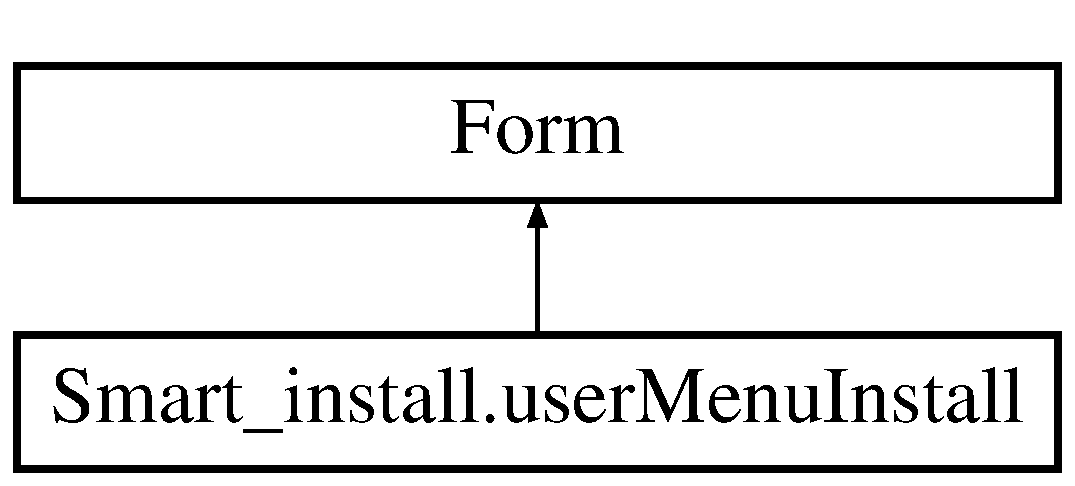
\includegraphics[height=2.000000cm]{class_smart__install_1_1user_menu_install}
\end{center}
\end{figure}
\subsection*{Metody publiczne}
\begin{DoxyCompactItemize}
\item 
\hyperlink{class_smart__install_1_1user_menu_install_a102223575d41f3e6c66438621e911678}{user\+Menu\+Install} ()
\end{DoxyCompactItemize}
\subsection*{Metody chronione}
\begin{DoxyCompactItemize}
\item 
override void \hyperlink{class_smart__install_1_1user_menu_install_ab9c936c4dba89e7311daa746dfcece7f}{Dispose} (bool disposing)
\begin{DoxyCompactList}\small\item\em Clean up any resources being used. \end{DoxyCompactList}\end{DoxyCompactItemize}


\subsection{Opis szczegółowy}


Definicja w linii 14 pliku user\+Menu\+Install.\+cs.



\subsection{Dokumentacja konstruktora i destruktora}
\hypertarget{class_smart__install_1_1user_menu_install_a102223575d41f3e6c66438621e911678}{\index{Smart\+\_\+install\+::user\+Menu\+Install@{Smart\+\_\+install\+::user\+Menu\+Install}!user\+Menu\+Install@{user\+Menu\+Install}}
\index{user\+Menu\+Install@{user\+Menu\+Install}!Smart\+\_\+install\+::user\+Menu\+Install@{Smart\+\_\+install\+::user\+Menu\+Install}}
\subsubsection[{user\+Menu\+Install}]{\setlength{\rightskip}{0pt plus 5cm}Smart\+\_\+install.\+user\+Menu\+Install.\+user\+Menu\+Install (
\begin{DoxyParamCaption}
{}
\end{DoxyParamCaption}
)}}\label{class_smart__install_1_1user_menu_install_a102223575d41f3e6c66438621e911678}


Definicja w linii 17 pliku user\+Menu\+Install.\+cs.



\subsection{Dokumentacja funkcji składowych}
\hypertarget{class_smart__install_1_1user_menu_install_ab9c936c4dba89e7311daa746dfcece7f}{\index{Smart\+\_\+install\+::user\+Menu\+Install@{Smart\+\_\+install\+::user\+Menu\+Install}!Dispose@{Dispose}}
\index{Dispose@{Dispose}!Smart\+\_\+install\+::user\+Menu\+Install@{Smart\+\_\+install\+::user\+Menu\+Install}}
\subsubsection[{Dispose}]{\setlength{\rightskip}{0pt plus 5cm}override void Smart\+\_\+install.\+user\+Menu\+Install.\+Dispose (
\begin{DoxyParamCaption}
\item[{bool}]{disposing}
\end{DoxyParamCaption}
)\hspace{0.3cm}{\ttfamily [protected]}}}\label{class_smart__install_1_1user_menu_install_ab9c936c4dba89e7311daa746dfcece7f}


Clean up any resources being used. 


\begin{DoxyParams}{Parametry}
{\em disposing} & true if managed resources should be disposed; otherwise, false.\\
\hline
\end{DoxyParams}


Definicja w linii 14 pliku user\+Menu\+Install.\+Designer.\+cs.



Dokumentacja dla tej klasy została wygenerowana z plików\+:\begin{DoxyCompactItemize}
\item 
\hyperlink{user_menu_install_8cs}{user\+Menu\+Install.\+cs}\item 
\hyperlink{user_menu_install_8_designer_8cs}{user\+Menu\+Install.\+Designer.\+cs}\end{DoxyCompactItemize}

\hypertarget{class_smart__install_1_1zip_creator}{\section{Dokumentacja klasy Smart\+\_\+install.\+zip\+Creator}
\label{class_smart__install_1_1zip_creator}\index{Smart\+\_\+install.\+zip\+Creator@{Smart\+\_\+install.\+zip\+Creator}}
}
\subsection*{Statyczne metody publiczne}
\begin{DoxyCompactItemize}
\item 
static void \hyperlink{class_smart__install_1_1zip_creator_ada007dd010892ba93dcfd65b65837669}{create\+Archive} (string destiny\+Path, string file\+Path)
\item 
static void \hyperlink{class_smart__install_1_1zip_creator_ad35072421dbf133168925d86702301e8}{add\+To\+Archive} (string to\+Add, string where\+Add, string name)
\item 
static void \hyperlink{class_smart__install_1_1zip_creator_a4f4fa6e6b2fe6ab6ddd4333778413ae3}{delete\+File} (string path)
\begin{DoxyCompactList}\small\item\em Usuwa wskazy plik z dysku \end{DoxyCompactList}\item 
static void \hyperlink{class_smart__install_1_1zip_creator_ab73cd9a014551fe63502f9e87e2d0bc5}{unzip\+File\+From\+Archive} (string file\+Path, string extract\+Path)
\item 
static string \hyperlink{class_smart__install_1_1zip_creator_a5dc6db46d832a7059272b8f81ef9df79}{get\+File} (string path, string name)
\item 
static void \hyperlink{class_smart__install_1_1zip_creator_ac6c7d6f4c0c0831a788c6cbd6ddd866c}{copy\+Between\+Archive} (string destiny\+Path, string source\+Path, string source\+File)
\end{DoxyCompactItemize}


\subsection{Opis szczegółowy}


Definicja w linii 11 pliku zip\+Creator.\+cs.



\subsection{Dokumentacja funkcji składowych}
\hypertarget{class_smart__install_1_1zip_creator_ad35072421dbf133168925d86702301e8}{\index{Smart\+\_\+install\+::zip\+Creator@{Smart\+\_\+install\+::zip\+Creator}!add\+To\+Archive@{add\+To\+Archive}}
\index{add\+To\+Archive@{add\+To\+Archive}!Smart\+\_\+install\+::zip\+Creator@{Smart\+\_\+install\+::zip\+Creator}}
\subsubsection[{add\+To\+Archive}]{\setlength{\rightskip}{0pt plus 5cm}static void Smart\+\_\+install.\+zip\+Creator.\+add\+To\+Archive (
\begin{DoxyParamCaption}
\item[{string}]{to\+Add, }
\item[{string}]{where\+Add, }
\item[{string}]{name}
\end{DoxyParamCaption}
)\hspace{0.3cm}{\ttfamily [static]}}}\label{class_smart__install_1_1zip_creator_ad35072421dbf133168925d86702301e8}





\begin{DoxyParams}{Parametry}
{\em to\+Add} & co dodajemy\\
\hline
{\em where\+Add} & gdzie dodajemy\\
\hline
{\em name} & nazwa pliku\\
\hline
\end{DoxyParams}


Definicja w linii 34 pliku zip\+Creator.\+cs.

\hypertarget{class_smart__install_1_1zip_creator_ac6c7d6f4c0c0831a788c6cbd6ddd866c}{\index{Smart\+\_\+install\+::zip\+Creator@{Smart\+\_\+install\+::zip\+Creator}!copy\+Between\+Archive@{copy\+Between\+Archive}}
\index{copy\+Between\+Archive@{copy\+Between\+Archive}!Smart\+\_\+install\+::zip\+Creator@{Smart\+\_\+install\+::zip\+Creator}}
\subsubsection[{copy\+Between\+Archive}]{\setlength{\rightskip}{0pt plus 5cm}static void Smart\+\_\+install.\+zip\+Creator.\+copy\+Between\+Archive (
\begin{DoxyParamCaption}
\item[{string}]{destiny\+Path, }
\item[{string}]{source\+Path, }
\item[{string}]{source\+File}
\end{DoxyParamCaption}
)\hspace{0.3cm}{\ttfamily [static]}}}\label{class_smart__install_1_1zip_creator_ac6c7d6f4c0c0831a788c6cbd6ddd866c}





\begin{DoxyParams}{Parametry}
{\em destiny\+Path} & sciezka archiwum, do którego kopiujemy\\
\hline
{\em source\+Path} & źródło archwium do któego kopiujemy\\
\hline
{\em source\+File} & nazwa pliku archwium źródłowego\\
\hline
\end{DoxyParams}


Definicja w linii 103 pliku zip\+Creator.\+cs.

\hypertarget{class_smart__install_1_1zip_creator_ada007dd010892ba93dcfd65b65837669}{\index{Smart\+\_\+install\+::zip\+Creator@{Smart\+\_\+install\+::zip\+Creator}!create\+Archive@{create\+Archive}}
\index{create\+Archive@{create\+Archive}!Smart\+\_\+install\+::zip\+Creator@{Smart\+\_\+install\+::zip\+Creator}}
\subsubsection[{create\+Archive}]{\setlength{\rightskip}{0pt plus 5cm}static void Smart\+\_\+install.\+zip\+Creator.\+create\+Archive (
\begin{DoxyParamCaption}
\item[{string}]{destiny\+Path, }
\item[{string}]{file\+Path}
\end{DoxyParamCaption}
)\hspace{0.3cm}{\ttfamily [static]}}}\label{class_smart__install_1_1zip_creator_ada007dd010892ba93dcfd65b65837669}





\begin{DoxyParams}{Parametry}
{\em name} & Nazwa archiwum\\
\hline
{\em destiny\+Path} & Gdzie ma powstać\\
\hline
{\em file\+Path} & nazwa zip\\
\hline
\end{DoxyParams}


Definicja w linii 19 pliku zip\+Creator.\+cs.

\hypertarget{class_smart__install_1_1zip_creator_a4f4fa6e6b2fe6ab6ddd4333778413ae3}{\index{Smart\+\_\+install\+::zip\+Creator@{Smart\+\_\+install\+::zip\+Creator}!delete\+File@{delete\+File}}
\index{delete\+File@{delete\+File}!Smart\+\_\+install\+::zip\+Creator@{Smart\+\_\+install\+::zip\+Creator}}
\subsubsection[{delete\+File}]{\setlength{\rightskip}{0pt plus 5cm}static void Smart\+\_\+install.\+zip\+Creator.\+delete\+File (
\begin{DoxyParamCaption}
\item[{string}]{path}
\end{DoxyParamCaption}
)\hspace{0.3cm}{\ttfamily [static]}}}\label{class_smart__install_1_1zip_creator_a4f4fa6e6b2fe6ab6ddd4333778413ae3}


Usuwa wskazy plik z dysku 


\begin{DoxyParams}{Parametry}
{\em path} & sciezka do usuwanego pliku\\
\hline
\end{DoxyParams}


Definicja w linii 46 pliku zip\+Creator.\+cs.

\hypertarget{class_smart__install_1_1zip_creator_a5dc6db46d832a7059272b8f81ef9df79}{\index{Smart\+\_\+install\+::zip\+Creator@{Smart\+\_\+install\+::zip\+Creator}!get\+File@{get\+File}}
\index{get\+File@{get\+File}!Smart\+\_\+install\+::zip\+Creator@{Smart\+\_\+install\+::zip\+Creator}}
\subsubsection[{get\+File}]{\setlength{\rightskip}{0pt plus 5cm}static string Smart\+\_\+install.\+zip\+Creator.\+get\+File (
\begin{DoxyParamCaption}
\item[{string}]{path, }
\item[{string}]{name}
\end{DoxyParamCaption}
)\hspace{0.3cm}{\ttfamily [static]}}}\label{class_smart__install_1_1zip_creator_a5dc6db46d832a7059272b8f81ef9df79}





\begin{DoxyParams}{Parametry}
{\em path} & sciezka do archiwum\\
\hline
{\em name} & nazwa wyodrebnionego pliku\\
\hline
\end{DoxyParams}
\begin{DoxyReturn}{Zwraca}

\end{DoxyReturn}


Definicja w linii 81 pliku zip\+Creator.\+cs.

\hypertarget{class_smart__install_1_1zip_creator_ab73cd9a014551fe63502f9e87e2d0bc5}{\index{Smart\+\_\+install\+::zip\+Creator@{Smart\+\_\+install\+::zip\+Creator}!unzip\+File\+From\+Archive@{unzip\+File\+From\+Archive}}
\index{unzip\+File\+From\+Archive@{unzip\+File\+From\+Archive}!Smart\+\_\+install\+::zip\+Creator@{Smart\+\_\+install\+::zip\+Creator}}
\subsubsection[{unzip\+File\+From\+Archive}]{\setlength{\rightskip}{0pt plus 5cm}static void Smart\+\_\+install.\+zip\+Creator.\+unzip\+File\+From\+Archive (
\begin{DoxyParamCaption}
\item[{string}]{file\+Path, }
\item[{string}]{extract\+Path}
\end{DoxyParamCaption}
)\hspace{0.3cm}{\ttfamily [static]}}}\label{class_smart__install_1_1zip_creator_ab73cd9a014551fe63502f9e87e2d0bc5}





\begin{DoxyParams}{Parametry}
{\em file\+Path} & nazwa zip\\
\hline
{\em extract\+Path} & nazwa po rozpakowaniu\\
\hline
\end{DoxyParams}


Definicja w linii 56 pliku zip\+Creator.\+cs.



Dokumentacja dla tej klasy została wygenerowana z pliku\+:\begin{DoxyCompactItemize}
\item 
\hyperlink{zip_creator_8cs}{zip\+Creator.\+cs}\end{DoxyCompactItemize}

\chapter{Dokumentacja plików}
\hypertarget{_add_programs_8cs}{\section{Dokumentacja pliku Add\+Programs.\+cs}
\label{_add_programs_8cs}\index{Add\+Programs.\+cs@{Add\+Programs.\+cs}}
}
\subsection*{Komponenty}
\begin{DoxyCompactItemize}
\item 
class \hyperlink{class_smart__install_1_1_add_programs}{Smart\+\_\+install.\+Add\+Programs}
\end{DoxyCompactItemize}
\subsection*{Przestrzenie nazw}
\begin{DoxyCompactItemize}
\item 
package \hyperlink{namespace_smart__install}{Smart\+\_\+install}
\end{DoxyCompactItemize}

\hypertarget{_add_programs_8_designer_8cs}{\section{Dokumentacja pliku Add\+Programs.\+Designer.\+cs}
\label{_add_programs_8_designer_8cs}\index{Add\+Programs.\+Designer.\+cs@{Add\+Programs.\+Designer.\+cs}}
}
\subsection*{Komponenty}
\begin{DoxyCompactItemize}
\item 
class \hyperlink{class_smart__install_1_1_add_programs}{Smart\+\_\+install.\+Add\+Programs}
\end{DoxyCompactItemize}
\subsection*{Przestrzenie nazw}
\begin{DoxyCompactItemize}
\item 
package \hyperlink{namespace_smart__install}{Smart\+\_\+install}
\end{DoxyCompactItemize}

\hypertarget{_archive_8cs}{\section{Dokumentacja pliku Archive.\+cs}
\label{_archive_8cs}\index{Archive.\+cs@{Archive.\+cs}}
}
\subsection*{Komponenty}
\begin{DoxyCompactItemize}
\item 
class \hyperlink{class_smart__install_1_1_archive}{Smart\+\_\+install.\+Archive}
\end{DoxyCompactItemize}
\subsection*{Przestrzenie nazw}
\begin{DoxyCompactItemize}
\item 
package \hyperlink{namespace_smart__install}{Smart\+\_\+install}
\end{DoxyCompactItemize}

\hypertarget{control_8cs}{\section{Dokumentacja pliku control.\+cs}
\label{control_8cs}\index{control.\+cs@{control.\+cs}}
}
\subsection*{Komponenty}
\begin{DoxyCompactItemize}
\item 
class \hyperlink{class_smart__install_1_1archive_information}{Smart\+\_\+install.\+archive\+Information}
\begin{DoxyCompactList}\small\item\em Klasa reprezentująca informację na temat archiwum uzyskiwane od urzytkownika \end{DoxyCompactList}\item 
class \hyperlink{class_smart__install_1_1program_information}{Smart\+\_\+install.\+program\+Information}
\begin{DoxyCompactList}\small\item\em Klasa reprezentująca informację na temat programu uzyskiwane od użytkownika \end{DoxyCompactList}\item 
class \hyperlink{class_smart__install_1_1control}{Smart\+\_\+install.\+control}
\end{DoxyCompactItemize}
\subsection*{Przestrzenie nazw}
\begin{DoxyCompactItemize}
\item 
package \hyperlink{namespace_smart__install}{Smart\+\_\+install}
\end{DoxyCompactItemize}

\hypertarget{_exec_8cs}{\section{Dokumentacja pliku Exec.\+cs}
\label{_exec_8cs}\index{Exec.\+cs@{Exec.\+cs}}
}
\subsection*{Komponenty}
\begin{DoxyCompactItemize}
\item 
class \hyperlink{class_smart__install_1_1_exec}{Smart\+\_\+install.\+Exec}
\end{DoxyCompactItemize}
\subsection*{Przestrzenie nazw}
\begin{DoxyCompactItemize}
\item 
package \hyperlink{namespace_smart__install}{Smart\+\_\+install}
\end{DoxyCompactItemize}

\hypertarget{_help2_8cs}{\section{Dokumentacja pliku Help2.\+cs}
\label{_help2_8cs}\index{Help2.\+cs@{Help2.\+cs}}
}
\subsection*{Komponenty}
\begin{DoxyCompactItemize}
\item 
class \hyperlink{class_smart__install_1_1_help2}{Smart\+\_\+install.\+Help2}
\end{DoxyCompactItemize}
\subsection*{Przestrzenie nazw}
\begin{DoxyCompactItemize}
\item 
package \hyperlink{namespace_smart__install}{Smart\+\_\+install}
\end{DoxyCompactItemize}

\hypertarget{_help2_8_designer_8cs}{\section{Dokumentacja pliku Help2.\+Designer.\+cs}
\label{_help2_8_designer_8cs}\index{Help2.\+Designer.\+cs@{Help2.\+Designer.\+cs}}
}
\subsection*{Komponenty}
\begin{DoxyCompactItemize}
\item 
class \hyperlink{class_smart__install_1_1_help2}{Smart\+\_\+install.\+Help2}
\end{DoxyCompactItemize}
\subsection*{Przestrzenie nazw}
\begin{DoxyCompactItemize}
\item 
package \hyperlink{namespace_smart__install}{Smart\+\_\+install}
\end{DoxyCompactItemize}

\hypertarget{_language_8cs}{\section{Dokumentacja pliku Language.\+cs}
\label{_language_8cs}\index{Language.\+cs@{Language.\+cs}}
}
\subsection*{Komponenty}
\begin{DoxyCompactItemize}
\item 
class \hyperlink{class_smart__install_1_1_language}{Smart\+\_\+install.\+Language}
\end{DoxyCompactItemize}
\subsection*{Przestrzenie nazw}
\begin{DoxyCompactItemize}
\item 
package \hyperlink{namespace_smart__install}{Smart\+\_\+install}
\end{DoxyCompactItemize}

\hypertarget{_menu_install_8cs}{\section{Dokumentacja pliku Menu\+Install.\+cs}
\label{_menu_install_8cs}\index{Menu\+Install.\+cs@{Menu\+Install.\+cs}}
}
\subsection*{Komponenty}
\begin{DoxyCompactItemize}
\item 
class \hyperlink{class_smart__install_1_1_menu_install}{Smart\+\_\+install.\+Menu\+Install}
\end{DoxyCompactItemize}
\subsection*{Przestrzenie nazw}
\begin{DoxyCompactItemize}
\item 
package \hyperlink{namespace_smart__install}{Smart\+\_\+install}
\end{DoxyCompactItemize}

\hypertarget{_menu_install_8_designer_8cs}{\section{Dokumentacja pliku Menu\+Install.\+Designer.\+cs}
\label{_menu_install_8_designer_8cs}\index{Menu\+Install.\+Designer.\+cs@{Menu\+Install.\+Designer.\+cs}}
}
\subsection*{Komponenty}
\begin{DoxyCompactItemize}
\item 
class \hyperlink{class_smart__install_1_1_menu_install}{Smart\+\_\+install.\+Menu\+Install}
\end{DoxyCompactItemize}
\subsection*{Przestrzenie nazw}
\begin{DoxyCompactItemize}
\item 
package \hyperlink{namespace_smart__install}{Smart\+\_\+install}
\end{DoxyCompactItemize}

\hypertarget{_model_archive_8_context_8cs}{\section{Dokumentacja pliku Model\+Archive.\+Context.\+cs}
\label{_model_archive_8_context_8cs}\index{Model\+Archive.\+Context.\+cs@{Model\+Archive.\+Context.\+cs}}
}
\subsection*{Komponenty}
\begin{DoxyCompactItemize}
\item 
class \hyperlink{class_smart__install_1_1_archive_base_entities2}{Smart\+\_\+install.\+Archive\+Base\+Entities2}
\end{DoxyCompactItemize}
\subsection*{Przestrzenie nazw}
\begin{DoxyCompactItemize}
\item 
package \hyperlink{namespace_smart__install}{Smart\+\_\+install}
\end{DoxyCompactItemize}

\hypertarget{_model_archive_8cs}{\section{Dokumentacja pliku Model\+Archive.\+cs}
\label{_model_archive_8cs}\index{Model\+Archive.\+cs@{Model\+Archive.\+cs}}
}

\hypertarget{_model_archive_8_designer_8cs}{\section{Dokumentacja pliku Model\+Archive.\+Designer.\+cs}
\label{_model_archive_8_designer_8cs}\index{Model\+Archive.\+Designer.\+cs@{Model\+Archive.\+Designer.\+cs}}
}

\hypertarget{_new_arch_8cs}{\section{Dokumentacja pliku New\+Arch.\+cs}
\label{_new_arch_8cs}\index{New\+Arch.\+cs@{New\+Arch.\+cs}}
}
\subsection*{Komponenty}
\begin{DoxyCompactItemize}
\item 
class \hyperlink{class_smart__install_1_1_new_arch}{Smart\+\_\+install.\+New\+Arch}
\end{DoxyCompactItemize}
\subsection*{Przestrzenie nazw}
\begin{DoxyCompactItemize}
\item 
package \hyperlink{namespace_smart__install}{Smart\+\_\+install}
\end{DoxyCompactItemize}

\hypertarget{_new_arch_8_designer_8cs}{\section{Dokumentacja pliku New\+Arch.\+Designer.\+cs}
\label{_new_arch_8_designer_8cs}\index{New\+Arch.\+Designer.\+cs@{New\+Arch.\+Designer.\+cs}}
}
\subsection*{Komponenty}
\begin{DoxyCompactItemize}
\item 
class \hyperlink{class_smart__install_1_1_new_arch}{Smart\+\_\+install.\+New\+Arch}
\end{DoxyCompactItemize}
\subsection*{Przestrzenie nazw}
\begin{DoxyCompactItemize}
\item 
package \hyperlink{namespace_smart__install}{Smart\+\_\+install}
\end{DoxyCompactItemize}

\hypertarget{_prog_8cs}{\section{Dokumentacja pliku Prog.\+cs}
\label{_prog_8cs}\index{Prog.\+cs@{Prog.\+cs}}
}
\subsection*{Komponenty}
\begin{DoxyCompactItemize}
\item 
class \hyperlink{class_smart__install_1_1_prog}{Smart\+\_\+install.\+Prog}
\end{DoxyCompactItemize}
\subsection*{Przestrzenie nazw}
\begin{DoxyCompactItemize}
\item 
package \hyperlink{namespace_smart__install}{Smart\+\_\+install}
\end{DoxyCompactItemize}

\hypertarget{_search_program_8cs}{\section{Dokumentacja pliku Search\+Program.\+cs}
\label{_search_program_8cs}\index{Search\+Program.\+cs@{Search\+Program.\+cs}}
}
\subsection*{Komponenty}
\begin{DoxyCompactItemize}
\item 
class \hyperlink{class_smart__install_1_1_search_program}{Smart\+\_\+install.\+Search\+Program}
\item 
struct \hyperlink{struct_smart__install_1_1_search_program_1_1_install_program}{Smart\+\_\+install.\+Search\+Program.\+Install\+Program}
\end{DoxyCompactItemize}
\subsection*{Przestrzenie nazw}
\begin{DoxyCompactItemize}
\item 
package \hyperlink{namespace_smart__install}{Smart\+\_\+install}
\end{DoxyCompactItemize}

\hypertarget{system_type_8cs}{\section{Dokumentacja pliku system\+Type.\+cs}
\label{system_type_8cs}\index{system\+Type.\+cs@{system\+Type.\+cs}}
}
\subsection*{Komponenty}
\begin{DoxyCompactItemize}
\item 
class \hyperlink{class_smart__install_1_1system_type}{Smart\+\_\+install.\+system\+Type}
\end{DoxyCompactItemize}
\subsection*{Przestrzenie nazw}
\begin{DoxyCompactItemize}
\item 
package \hyperlink{namespace_smart__install}{Smart\+\_\+install}
\end{DoxyCompactItemize}

\hypertarget{_tag_8cs}{\section{Dokumentacja pliku Tag.\+cs}
\label{_tag_8cs}\index{Tag.\+cs@{Tag.\+cs}}
}
\subsection*{Komponenty}
\begin{DoxyCompactItemize}
\item 
class \hyperlink{class_smart__install_1_1_tag}{Smart\+\_\+install.\+Tag}
\end{DoxyCompactItemize}
\subsection*{Przestrzenie nazw}
\begin{DoxyCompactItemize}
\item 
package \hyperlink{namespace_smart__install}{Smart\+\_\+install}
\end{DoxyCompactItemize}

\hypertarget{user_menu_install_8cs}{\section{Dokumentacja pliku user\+Menu\+Install.\+cs}
\label{user_menu_install_8cs}\index{user\+Menu\+Install.\+cs@{user\+Menu\+Install.\+cs}}
}
\subsection*{Komponenty}
\begin{DoxyCompactItemize}
\item 
class \hyperlink{class_smart__install_1_1user_menu_install}{Smart\+\_\+install.\+user\+Menu\+Install}
\end{DoxyCompactItemize}
\subsection*{Przestrzenie nazw}
\begin{DoxyCompactItemize}
\item 
package \hyperlink{namespace_smart__install}{Smart\+\_\+install}
\end{DoxyCompactItemize}

\hypertarget{user_menu_install_8_designer_8cs}{\section{Dokumentacja pliku user\+Menu\+Install.\+Designer.\+cs}
\label{user_menu_install_8_designer_8cs}\index{user\+Menu\+Install.\+Designer.\+cs@{user\+Menu\+Install.\+Designer.\+cs}}
}
\subsection*{Komponenty}
\begin{DoxyCompactItemize}
\item 
class \hyperlink{class_smart__install_1_1user_menu_install}{Smart\+\_\+install.\+user\+Menu\+Install}
\end{DoxyCompactItemize}
\subsection*{Przestrzenie nazw}
\begin{DoxyCompactItemize}
\item 
package \hyperlink{namespace_smart__install}{Smart\+\_\+install}
\end{DoxyCompactItemize}

\hypertarget{zip_creator_8cs}{\section{Dokumentacja pliku zip\+Creator.\+cs}
\label{zip_creator_8cs}\index{zip\+Creator.\+cs@{zip\+Creator.\+cs}}
}
\subsection*{Komponenty}
\begin{DoxyCompactItemize}
\item 
class \hyperlink{class_smart__install_1_1zip_creator}{Smart\+\_\+install.\+zip\+Creator}
\end{DoxyCompactItemize}
\subsection*{Przestrzenie nazw}
\begin{DoxyCompactItemize}
\item 
package \hyperlink{namespace_smart__install}{Smart\+\_\+install}
\end{DoxyCompactItemize}

%--- End generated contents ---

% Index
\newpage
\phantomsection
\addcontentsline{toc}{chapter}{Indeks}
\printindex

\end{document}
